\documentclass[12pt]{article}
\usepackage{amsthm}
\usepackage{textcomp}
\usepackage[utf8]{inputenc}
\usepackage[english]{babel}
\usepackage{amssymb}
\usepackage{amsmath}
\usepackage{comment}
\usepackage{appendix}
\usepackage{graphicx}
\usepackage{pdfpages}
\usepackage[font=scriptsize]{caption}
\usepackage{mwe}
\graphicspath{ {Figures/} }
\usepackage{listings}
\usepackage{xcolor}
%New colors defined below
\definecolor{codegreen}{rgb}{0,0.6,0}
\definecolor{codegray}{rgb}{0.5,0.5,0.5}
\definecolor{codepurple}{rgb}{0.58,0,0.82}
\definecolor{backcolour}{rgb}{0.95,0.95,0.92}

%Code listing style named "mystyle"
\lstdefinestyle{mystyle}{
  backgroundcolor=\color{backcolour},   commentstyle=\color{codegreen},
  keywordstyle=\color{magenta},
  numberstyle=\tiny\color{codegray},
  stringstyle=\color{codepurple},
  basicstyle=\ttfamily\footnotesize,
  breakatwhitespace=false,         
  breaklines=true,                 
  captionpos=b,                    
  keepspaces=true,                 
  numbers=left,                    
  numbersep=5pt,                  
  showspaces=false,                
  showstringspaces=false,
  showtabs=false,                  
  tabsize=2
}

%"mystyle" code listing set
\lstset{style=mystyle}
\usepackage{xcolor}
\DeclareMathOperator{\Tr}{Tr}
\DeclareMathOperator{\Det}{Det}
\newtheorem{theorem}{Theorem}[section]
\newtheorem{definition}{Definition}[section]
\newtheorem{lemma}{Lemma}[section]
\title{Pattern Formation in Stochastic Partial Differential Equations}
\author{Joseph W. Shingleton }
\usepackage[
style=numeric
]{biblatex}
\addbibresource{Dissertation.bib}
\usepackage


\begin{document}
\includepdf[pages=-]{Declaration.pdf}
\maketitle
\newpage
\section*{Acknowledgements}
I would like to thank my supervisor, Dr. Mariya Ptashnyk, whose encouragement, guidance and advice has been instrumental in the development of this Dissertation. I would also like to thank Prof. Kevin Painter, whose insightful questioning elucidated new paths of investigation for the study.  
\newpage
\section*{Abstract}
Turing's celebrated 1952 work on pattern formation came with a single central paradox: how can the dissipative force of diffusion be the root of spatial structure in a system? Recent studies into the effects of stochastic noise on pattern forming systems have lead to equally unlikely results. This dissertation attempts to demonstrate the potential for stochastic noise to be a creative force within such systems. We begin by demonstrating the well-posedness of two deterministic models, the \textit{Schakenberg} and \textit{Gierer-Meinhardt} models, before extending this analysis to similar systems with both multiplicative and additive demographic white-noise. We then implement a method for simulating stochastic reaction diffusion systems, and show that patterning can occur outside of the parameter range expected from deterministic systems. We also show that stochastic patterns formed just within the deterministically permitted range often develop more quickly, and are more intense, than their deterministic counterparts. Furthermore, we demonstrate that demographic white-noise alone can not account for mode-shifting behaviour in pattern forming systems, and that we must consider stochastic forcing of parameters to achieve such results. By doing so, we are able to achieve patterning which is qualitatively similar to that of biological systems.  
\newpage
\tableofcontents
\newpage
\section{Introduction}
The spontaneous formation of spatial patterns from an otherwise homogenous medium is a key problem in many areas of science, and in particular in biology. At first glance, the emergence of structure from chaos appears to directly contradict the entropic principles of thermodynamics, and yet it is a process which consistently occurs in biological systems. 

The first attempts to provide a mathematical explanation for this process came from Alan Turing in 1952. Turing showed that the diffusion of two interacting chemicals can drive the development of spatially distributed patterns, going on to suggest that this process could explain the morphogenesis seen in embryonic development \cite{Turing}. Turing's revolutionary idea, that the usually homogenising force of diffusion could in fact drive the development of spatial heterogeneity, has gone on to become one of the corner-stone models of theoretical biology, with applications as diverse as modelling the distribution of organisms in an ecosystem (e.g. \cite{Wilson}), the spread of infectious diseases (e.g. \cite{Wang}), and even in the signals processed by neurological networks \cite{Froese}.   

However, deterministic Turing pattern formation is not without its limitations. Such mechanisms frequently fail to capture the uncertain, messy nature of biological systems. Moreover, the partial differential equations which form the basis of the theory are reliant on the mean field approximation. In cases where one species is of a much higher relative density than another, which is often the case in bio-chemical processes, this approximation breaks down, and we must consider the effect of demographic white-noise on the system \cite{Dewar}.  

Furthermore, the parametric constraints of Turing bifurcation are often unreasonably restrictive. Turing analysis dictates that pattern formation will only occur if the ratio between the diffusivity rates of interacting species is sufficiently high \cite{Murray}. While this is frequently achieved in systems with diffusing chemicals (e.g. in developmental biology), it is often not the case in ecological systems \cite{Karig, Butler}. However, despite this restriction, we often still observe Turing like patterns in these systems. In \cite{Butler} it is shown that these early Turing patterns, or \textit{quasipatterns}, can be achieved via the introduction of demographic white-noise. A further example of this phenomenon is demonstrated in \cite{Biancalani}, in which quasipatterns are shown to develop in a stochastic Brusselator model.   

Modelling the changes in modal frequency often seen in biological patterning has also been a challenge for researchers. The process can be replicated in a deterministic Turing system by allowing the domain to grow during the simulation (e.g. \cite{Crampin}), which is sufficient for explaining mode changes in, for example, embryo development, but cannot explain changes in systems with a fixed domain. An alternate avenue of research for this problem has been \textit{random partial differential equation}, in which a given parameter is permitted to have some stochastic variance, as opposed to the demographic stochasticity described above \cite{Zhonghuai}.

This dissertation aims to present a detailed investigation into the properties of systems of pattern forming stochastic partial differential equations. Particular attention will be payed to the systems with demographic white-noise, as these have the richest body of research, however stochastic forcing of parameters will also be investigated.

In Section 2 we will introduce two deterministic pattern forming systems, the Schnakenberg and Gierer-Meinhardt models. The existence of unique mild solutions will be demonstrated for these systems, and it will be shown, via the method of invariant sets, that such solutions are able to maintain positivity. 

Section 3 will investigate the stochastic counterparts of the same models. It will begin by introducing useful tools in the analysis of stochastic differential equations, before showing that, given proper constraints on the size of the stochastic noise, unique mild solutions exist for the Schnakenberg model, and for a modified version of the Gierer-Meinhardt model.

An algorithm for simulating stochastic partial differential equations will be presented in section 4. This will involve developing both a finite difference method for approximating deterministic PDEs, and a method for generating sample paths for stochastic processes.  

The pattern forming characteristics of deterministic systems will be analysed in section 5. In particular, we will identify the critical diffusivity parameter required for pattern formation to occur. These results will be compared against stochastic simulations of the same system in section 6. We will show that patterning is possible for sub-critical parameter values, and that these patterns lack the stability seen in deterministic systems. We will also see that stochastic systems are able to fall into strongly patterned states more quickly than identical deterministic systems.

Section 7 will investigate the effect of stochastic forcing of model parameters. The concept of a \textit{random partial differential equation} will be introduced, and their pattern forming properties will be studied. In particular, we will see that allowing the stochastic forcing to vary only in time produces symmetric patterns which spontaneously shift in modal frequency, and that these shifts have hysteric properties. Following this, we will show that by permitting the stochastic forcing to vary in both space and time, we are able to produce asymmetric patterns with fluid transitions between patterning regimes.

\section{An analysis of reaction-diffusion models}
Before approaching the problem of pattern formation in stochastic systems, it will first be necessary to lay out the mathematical groundwork for the problem in the deterministic case. This section will introduce two pattern forming models and investigate the well-posedness of each system, as prescribed in \cite{Lord}, along with the positivity of solutions as prescribed in \cite{Smoller}. A detailed investigation into the pattern forming characteristics of each system will be provided in \textsection 5, including analysis of the Turing bifurcation points and critical parameters in each model. The techniques used to formalise the deterministic problem in this section will, where appropriate, be applied to their stochastic counterparts in \textsection 3. 


This paper focuses solely on PDEs describing reaction-diffusion systems. For the purposes of this investigation, we will only be considering two-species interactions occurring in a single spatial dimension. The deterministic equations describing these reactions will take the form:

\begin{equation} \label{dpde1}
\frac{\partial u(x,t)}{\partial t} = D_1\Delta u(x,t) + f(u,v),
\end{equation}
\begin{equation} \label{dpde2}
\frac{\partial v(x,t)}{\partial t} = D_2\Delta v(x,t) + g(u,v),
\end{equation}
with $ x \in [0,L]$, $ t \in [0,T]$, $D_i \in \mathbb{R}^+$ for $i = 1,2$ and $f,g:\mathbb{R}^2\rightarrow\mathbb{R}$. Where appropriate, the vector $w = (u,v)^\intercal \in \mathbb{R}^2$ will be used, in such a case it is assumed that the non-linear function, $F(w)$, is also a two dimensional function.  The system is under non-homogeneous Neumann boundary conditions: 
$$
\frac{\partial{w(0,t)}}{\partial{x}} = \frac{\partial{w}(L,t)}{\partial{x}} = 0,$$
and initial conditions:
$$
w(x,0) = 
\begin{pmatrix}
u(x,0)\\
v(x,0)
\end{pmatrix}
=
\begin{pmatrix}
u_0\\
v_0
\end{pmatrix}.
$$

This dissertation will focus on two models: the \textit{Schnakenberg} model and a \textit{Gierer-Meinhardt} model. These models are characterised by the non-linear function $f(u,v)$ and $g(u,v)$. For the Schnakenberg model \cite{Schnakenberg} we have:

\begin{equation} \label{ScFunc}
f(u,v) = \gamma \cdot (a-u+u^2v), \quad g(u,v) = \gamma \cdot (b-u^2v),
\end{equation}
and for the Gierer-Meinhardt model \cite{Meinhardt} we have:
\begin{equation} \label{AIFunc}
f(u,v) = \gamma \cdot (a-bu+\frac{u^2}{v}), \quad g(u,v) = \gamma \cdot (u^2 - v).
\end{equation}

Where $a$ and $b$ are positive constants. The parameter $\gamma$ in (\ref{ScFunc} - \ref{AIFunc}) has the effect of scaling the model parameters \cite{Murray}. The mathematical analysis performed in this section will not be affected by $\gamma$, and as such we will assume $\gamma = 1$. In \textsection 7 we will return to this parameter, and see how it influences the mode selection of pattern forming systems. 

This section will explore the concept of a \textit{mild solution} to systems of differential equations. We will show that the standard procedure for proving the existence of unique mild solutions, as described in \cite{Lord}, will not be sufficient in this case. We will ultimately need to show that solutions remain inside an invariant set, employing a method described in \cite{Smoller}. 

\subsection{Important tools and concepts}
This section provides brief definitions of some of the important concepts used in the analysis of partial differential equations, including \textit{semigroups} and \textit{infinitesimal generators}, which will allow us to provide some intuition into the concept of a \textit{mild solution} to a PDE problem. Much of the analysis in the proceeding section is based on examples in \cite{Lord} and \cite{Pazy}, including the following definitions.

\begin{definition}[Semigroup] \label{SGprop} \cite{Lord, Pazy}
Consider a Banach space $X$. The operator $S(t):X\to X$ is a semigroup for $X$ if:
\begin{enumerate}
\item[(i)] $S(0) = I$,
\item[(ii)] $S(t+s) = S(t)S(s)$ for $s,t \geq 0$,
\end{enumerate}
where $I$ refers to the identity matrix.  
\end{definition}
\begin{definition}[Infinitesimal Generator] \cite{Lord, Pazy} \label{IGprop}
For a semigroup $S(t)$ acting on a phase space $X$, the infinitesimal generator $-A$ is defined by:

$$(-A)w:=\lim_{h \downarrow 0} \frac{S(h)w - w}{h}.$$
The set of $w \in X$ for which this limit exists is the domain of $-A$, denoted by $\mathcal{D}(A)$. 
\end{definition}


Identification of an \textit{infinitesimal operator} acting on a \textit{semigroup} is a key process in the formulation of a \textit{mild solution} to a PDE problem. By application of these techniques, one is able to treat PDE systems as ODE systems acting on a Banach space, $X$. To illustrate an application of this process, consider the following reaction-diffusion system:
\begin{equation}\label{RD}
\frac{\partial}{\partial t} w = \Delta w + F(w), \quad w(0,x) = w_0(x) \quad f: \mathbb{R} \to \mathbb{R},
\end{equation}
with Neumann boundary conditions on the domain $x \in \Omega$. The aim of semigroup theory is to take the solution $w(t,x)$, which depends on both position and time, and rewrite it as the function $w:[0,\infty) \to L^2(\Omega)$, where $L^2$ refers to the space of square integrable functions. To achieve this, we set $-A := \Delta$, giving us the following ODE:
\begin{equation}
\frac{d}{d t} w = -A w + F(w), \quad w(0) = w_0.
\end{equation}
However, since the phase space has now changed due to the action of the infinitesimal generator $-A$, we must also change the domain on which the problem is posed. We consider the Hilbert space $H^k(\Omega)$, denoting a space containing both an $H^k$ inner product and adhering to Neumann boundary conditions on $\Omega$. In particular, for this problem we require the domain $\mathcal{D}(A) = \lbrace u,v \in H^1(\Omega) \cap H^2_0(\Omega): \nabla u,v = 0 \quad \text{for} \quad u,v\in\Omega\rbrace$. Given the operator $-A$ has the corresponding semigroup $S(t)$, variation of constants provides us with the following \cite{Lord, Pazy}:
\begin{equation} \label{mildsol}
w(t) = S(t)w_0 + \int_0^t S(t-s)F(w(s))d s.
\end{equation}
This solution, known as a \textit{mild solution}, solves (\ref{dpde1}-\ref{dpde2}) for $t \in [0,T]$ and $w_0 \in H$. We will now show that unique mild solutions exist for the models above. In \textsection 3.2, we will see how the same approach can be used to define mild solutions for stochastic PDEs. 

\subsection{Well-posedness in deterministic PDEs}

The necessary conditions for a reaction diffusion system to have unique solutions are stated and proved in \cite{Jost} and \cite{Lord}. In order to motivate the techniques used to analyse the \textit{Schnakenberg} and \textit{Gierer-Meinhardt} models, an outline of the theorem and proof, as described in \cite{Lord}, is given below.

\begin{theorem}\cite{Lord}
Suppose $-A:\mathcal{D}(A)\subset H \to H$ is a linear operator acting on the Hilbert space $H$, and that the eigenvalues of $-A$ are such that it has an inverse. There exists a mild solution $w(t)$ of the form of \eqref{mildsol} for some initial data $w_0 \in H$ and some non-linear function $F:H\to H$, if $F$ obeys the linear growth condition and is Lipschitz continuous. That is, the following inequalities hold:
\begin{align}\label{continuity}
||F(w)|| &\leq L(1+||w||),\\
\label{Lipcont}
||F(w_1) - F(w_2)|| &\leq L||w_1-w_2||, \quad \forall \quad w_1, w_2 \in H.
\end{align}
There also exists a $K_T$ such that:
\begin{equation} \label{existence}
||w(t)|| \leq K_T(1+||w_0||), \quad 0\leq t\leq T.
\end{equation}
\end{theorem}
\begin{proof}
This proof follows closely to that provided in \cite{Lord}. First, we define $\mathcal{J}$ as the linear operator acting on $w$ which produces the mild solution \eqref{mildsol}, such that the fixed points of $\mathcal{J}$ will be solutions to \eqref{mildsol}. Hence, we have:
$$(\mathcal{J}w)(t):= S(t)w_0 + \int_0^tS(t-s)F(w(s))ds,$$

To prove that these solutions exist, it is then necessary to show that $\mathcal{J}$ is a contraction and that it maps onto the Bannach space $X:= C([0,T],H)$ with norm $||w||_X:=\sup_{0\leq t\leq T}||w(t)||$. 

For $w\in X$ we have $||\mathcal{J}w||_X := \sup_{t\in[0,T]}||(\mathcal{J}w)(t)|| < \infty$. Hence, since $\mathcal{J}w:[0,T]\to H$, we have $\mathcal{J}w \in X$. We may now consider the difference between $\mathcal{J}$ acting on $w_1$ and $w_2$, given by:
$$ ||\mathcal{J}w_1(t) - \mathcal{J}w_2(t)|| = \int_0^t||S(t-s)(F(w_1(s))-F(w_2(s)))||ds.$$
Application of \eqref{Lipcont}, and given that $S(t-s) < 1$ for all $t$ and $s$, we arrive at:
\begin{align*}
 ||\mathcal{J}w_1(t) - \mathcal{J}w_2(t)|| &\leq \int_0^tL||w_1(s)-w_2(s)||ds,\\
 &\leq LT||w_1 - w_2||, \quad 0\leq t\leq T.
\end{align*}
Hence $\mathcal{J}$ is a contraction if $LT<1$. To see that $\mathcal{J}$ also adheres to condition \eqref{existence}, we apply the triangle inequality, yielding:
\begin{align*}
||(\mathcal{J}w)(t)||&\leq ||S(t)w_0|| + ||\int_0^tS(t-s)F(w(s))ds||,\\
&\leq ||S(t)||\cdot ||w_0|| + \int_0^t ||S(t-s)||\cdot||F(w(s))||ds.
\end{align*}
 Again, given that $||S(t)||<1$ for all $t$, and that $||F(w(s)|| \leq L(1+||w(s)||)$, we arrive at the following:
\begin{equation*}
||\mathcal{J}w(t)||\leq||w_0|| + \int_0^t L(1 + ||w(s)||)ds.
\end{equation*}
Hence, we have:
$$||w(t)|| \leq ||w_0|| + \int_0^tL(1+||w(s)||)ds,$$
finally, application of Gr\"{o}nwall's inequality, gives us:
$$||w(t)|| \leq e^{LT}(||w_0|| + 1),$$
and so we have arrived at \eqref{existence} as required, with $K_T = e^{LT}$ \cite{Lord}. 
\end{proof}

In order to test the well posedness of the problem in the deterministic case we simply need to show that the function $f(u,v)$ and $g(u,v)$ are Lipschitz continuous for both systems. However, this comes with its own set of complications - namely the non-linearity of the functions involved. Consider the functions for the Schnakenberg system \eqref{ScFunc}:
$$ ||f(u_1, v_1) - f(u_2,v_2)|| = ||(a-u_1+u_2^2v_1)-(a-u_2+u_2^2v_2)||.$$
By the the triangle inequality we arrive at:
\begin{align*}
||f(u_1,v_1) - f(u_2,v_2)|| &\leq ||u_1 - u_2|| + ||u_1^2v_1 - u_2^2v_2||,\\
    &\leq ||u_1 - u_2|| + ||u_1^2v_1 - u_2^2v_2 + u_1^2v_2 - u_1^2v_2||,\\
    &\leq ||u_1 - u_2|| + u_1^2||v_1 - v_2|| + v_2||u_1^2 - u_2^2||.
\end{align*}
So long as $u^2$ and $v$ are unbounded then we can not adhere to Theorem 2.1, so there is no unique mild solution. Similar analysis of the function $g(u,v)$ yields the following inequality:
$$ ||g(u_1,v_1) - g(u_2,v_2)|| \leq u_1^2||v_1 - v_2|| + v_1||u_1^2 - u_2^2||.$$

As such, it will be necessary to prove that the system contains an invariant set $\mathbf{\Sigma} = \lbrace (u,v) : 0\leq u \leq \alpha, 0\leq u \leq \beta\rbrace$ for some $\alpha, \beta < \infty$. This will ensure that any process with initial conditions $(u_0, v_0) \in \mathbf{\Sigma}$ will be bounded from above, satisfying the Lipschitz condition and indicating the existence of a unique mild solution.

Carrying out the same process with the Gierer-Meinhardt system provides even more restrictive conditions. Analysis of the non-linear functions in this case yields:
\begin{align*}
||f(u_1,v_1) - f(u_2,v_2)|| &\leq b||u_1 - u_2|| + u_1^2||\frac{1}{v_1} - \frac{1}{v_2}|| + \frac{1}{v_2}||u_1^2 - u_2^2||,\\
||g(u_1,v_1) - g(u_2,v_2)|| &\leq ||v_1 - v_2|| + u_1||u_1 - u_2||+ u_2||u_1 - u_2||.
\end{align*}
For this model to adhere to Lipschitz continuity we not only require that $u$ and $v$ are bounded from above but also that $v$ is strictly positive. Hence, for the system to have a unique mild solution we need to prove the existence of the invariant set $\mathbf{\Sigma} = \lbrace (u,v) : 0\leq u \leq \alpha, 0< v \leq \beta\rbrace$. The existence of such a set will be demonstrated below. 
\subsection{Positivity and boundedness of solutions}

As we saw in the previous section, it is important that we can prove that solutions to our systems remain bounded from above. However, when dealing with models approximating biological systems, it is also important that we can ensure the non-negativity of solutions - a solution describing a negative chemical concentration is of little use to a biologist. As such, we must ensure that any equations we use to model such systems can, at the very least, retain non-negativity for the time period and domain of the simulation. 
\newpage
\subsubsection{The method of invariant sets}
The method of invariant sets, as described by Smoller in \cite{Smoller}, provides a useful tool in assessing the positivity of reaction-diffusion systems. In addition, this method can also be employed to prove that the system has an upper bound which, as previously discussed, will be sufficient for showing that the problems are well posed.

The aim is to show that the set $\mathbf{\Sigma} = \lbrace (u,v): 0\leq u\leq\alpha, 0\leq v\leq\beta \rbrace$ is invariant for our systems. If such a set exists, then any solution starting inside $\mathbf{\Sigma}$ will remain bounded and non-negative. The method described in \cite{Smoller} is for the more general case of reaction diffusion systems with an additional advection term, however the same results apply for the reaction-diffusion systems studied in this dissertation. 

We first define the set of functions, $G_i(w)$, which make up the invariant set $\mathbf{\Sigma}$. Assume $w(x,t) \in \mathbb{R}^2$ is a solution to (\ref{dpde1}-\ref{dpde2}), with initial conditions $w(x,0) \in \mathbf{\Sigma}$, such that the solution at any time is $w(x,t)\in \mathbf{\Sigma}$. The set of functions $G_i(w)$ make up this invariant set $\mathbf{\Sigma}$, such that $G_i(w) < 0$ for all $w(x,t) \in \mathbf{\Sigma}$. 

We now consider what the functions $G_i(w)$ will look like in the case that our solutions do not stay inside $\mathbf{\Sigma}$. We have that, for some time $t=T$ and some point $x = x_0$:
  $$w(x_0,T) \notin \mathbf{\Sigma} \Longrightarrow G_i(w(x_0,T)) > 0.$$
If the initial conditions gave $w(x_0,0) \in \mathbf{\Sigma}$, then we must have that there exists some $0<t_0<T$ for which $G_i (w(x_0,t_0)) = 0$. It follows that we must have:
$$\frac{\partial{G_i(w(x,t))}}{\partial{t}} < 0 \quad \text{at} \quad (x_0,t_0).$$
Hence, if we can show that such functions exist, then we are able to show that $\mathbf{\Sigma}$ is an invariant set for our system \cite{Smoller}. Smoller provides us with the following test for this:
\begin{theorem}
Consider the following reaction diffusion system
$$w_t(x,t) = Dw_{xx}(x,t) + F(w(x,t)),$$
where $w_t(x,t)$ refers to the first time derivative of $w(x,t)$ and $w_{xx}(x,t)$ refers to the second spatial derivative of $w(x,t)$. Let $\mathbf{\Sigma}$ and $G_i$ be defined as above and define $\nabla G_i$ as the gradient of $G_i$, and $\mu$ as the eigenvalues of the matrix $D$.  For every $w_0 = w(x_0,t_0) \in \partial \mathbf{\Sigma}$, that is where $G_i(w_0) = 0$, let the following conditions hold:
\begin{enumerate}
\item [(i)]$\nabla G_i$ is a left eigenvector of $D$, so that $\nabla G_iD = \mu \nabla G_i$.
\item [(ii)] If $\nabla G_i(\xi) = 0$, then $\nabla^2G_i(\xi,\xi) \geq 0$.
\item [(iii)]$\nabla G_i(F(w_0))<0$ for all $t$. 
\end{enumerate}
Then $\mathbf{\Sigma}$ is an invariant set for the system. 
\end{theorem}
\begin{proof}

This proof is an outline of a more detailed proof provided by Smoller in \cite{Smoller}. First, we consider a point $(x_0,t_0)$. Given that at $(x_0,t_0)$ we have $G_i(w_0) = 0$, then from the chain rule we have:

$$\frac{\partial (G_i(w_0))}{\partial t} = \nabla G_i(w_t) = \nabla G_i(Dw_{xx}+F(w)).$$
Hence, by (i) we have that:
\begin{equation}\label{invproof}
\frac{\partial (G_i(w_0))}{\partial t} = \mu \nabla G_iw_{xx}+\nabla G_i(F(w)).
\end{equation}
Next, we define the functions:
$$h(x) = G_i(w(x_0,t_0)) = 0,$$ 
and its derivative 
$$h'(x) = \nabla G_i(w_x(x_0,t_0)).$$

Observe that if $h'(x_0) > 0$, then for $x > x_0$, where $x$ is close to $x_0$, we must have $h(x) > 0$. This implies that $G_i(w(x,t_0)) > 0$. Hence, for some $t$ close to $t_0$ we must have $G_i(w(x,t)) > 0$, contradicting the assumption that  $G_i(w(x,t))$ is negative for $w(x,t) \in \mathbf{\Sigma}$. Similarly if we take $h'(x_0) < 0$ and consider $x < x_0$ we arrive at the same contradiction, implying we must have: 
\begin{equation}\label{QCcond}
h'(x_0) = \nabla G_i(w_x(x,t_0)) = 0.
\end{equation}
In addition to this, if we have $h''(x_0)>0$ then we must also have $h(x)>0$ for some $x>x_0$, which we have already seen is impossible. Hence we are limited to $h''(x_0) \leq 0$. Application of the chain rule gives us:  
  
  $$h''(x_0) = \nabla^2G_i(w_x,w_x) + \nabla G_i(w_{xx}) \leq 0.$$
  
From (ii) and \eqref{QCcond} we have that  $\nabla^2G_i(w_x,w_x) \geq 0$, which implies that $\nabla G_i(w_{xx}) < 0$. Given that $D$ has only positive components, so that $\mu>0$, and considering \eqref{invproof} and condition (iii), we arrive at the required inequality:
$$\frac{\partial (G_i(w_0))}{\partial t} \leq \nabla G_i(F(w_0)) < 0.$$
\end{proof}

Finding the functions $G_i(w)$ is relatively straight forward. Condition (i) is arrived at easily when we consider that $D$ is a diagonal matrix, so any linear function $G_i(w)$ will satisfy the condition. The same conclusion is arrived at with condition (ii), as the second derivative of a linear function will be zero.  Condition (iii) requires that, for $V = \lbrace f(u,v),g(u,v)\rbrace$ on $(u,v)=\partial \mathbf{\Sigma}$, the inequality $\nabla G_i V \leq 0.$ holds. 

\subsubsection{Invariant sets of the Schnakenberg system}
To show that solutions to the Schnakenberg system \eqref{ScFunc} remain positive we let the vector $V   = \lbrace (a - u +u^2v), (b - u^2v) \rbrace $, and define the functions $G_1 = -u$ and $G_2 = -v$, giving the following conditions for $\mathbf{\Sigma} = \lbrace u, v : u\geq 0, v\geq 0 \rbrace$ to be an invariant region:

$$ \left. \nabla G_1 V \right|_{u=0} \leq 0 \Longleftrightarrow -a \leq 0,$$
$$ \left. \nabla G_2 V \right|_{v=0} \leq 0 \Longleftrightarrow -b \leq 0.$$

Since $a,b > 0$ these conditions must hold for all $u$ and $v$, so solutions retain non-negativity. 

We must also show that the region has an upper bound. This is achieved by considering the region $\mathbf{\Sigma} = \lbrace (u,v) : 0\leq u \leq \alpha, 0\leq v \leq \beta\rbrace$, and the functions $G_3 = u - \alpha$ and $G_4 = v - \beta$. This gives us the following inequalities:
\begin{align}
 \left. \nabla G_3 V \right|_{u=\alpha} &\leq 0 \Longleftrightarrow a -\alpha + \alpha^2v \leq 0,\\
\left. \nabla G_4 V \right|_{v=\beta} &\leq 0 \Longleftrightarrow b-u^2\beta \leq 0.
\end{align}
Since $v \leq \beta$, then for (11) to hold for all $v$, we must have:
$$a -\alpha + \alpha^2\beta \leq 0.$$
Then, by (12) we have:
$$a -\alpha + \alpha^2\frac{b}{u^2} \leq 0,$$
which, given that $0\leq u \leq \alpha \Longrightarrow u^2 \leq \alpha^2$, and by (12), gives us the following condition on $\alpha$ and $\beta$:
\begin{align*}
\alpha &\geq a+b,\\
\beta&\geq\frac{b}{(a+b)^2}.
\end{align*}
We can chose an $\alpha$ and $\beta$ satisfying these conditions such that for any $(u_0,v_0) \in \mathbf{\Sigma}$, the solution will remain within $\mathbf{\Sigma}$ and retain its non-negativity. Since these solutions are bounded we have that $f(u,v)$ and $g(u,v)$ are Lipschitz continuous and so a unique mild solution must exist for the Schnakenberg system. 

\subsubsection{Invariant sets of the Gierer-Meinhardt system}
As shown in \textsection 2.2, we require that the Gierer-Meinhardt system is not only non-negative, but also that it remains strictly positive. Hence, we will consider the invariant region $\mathbf{\Sigma} = \lbrace (u,v) : \delta \leq u \leq \alpha, \varepsilon \leq v \leq \beta\rbrace$. We set $V = \lbrace (a - bu + u^2/v),(u^2 - v)\rbrace$, and use the functions $G_1 = \delta - u$, $G_2 = \varepsilon - v$, $G_3 = u - \alpha$, and $G_4 = v - \beta$. This gives us:
\begin{align*}
    \left.\nabla G_1 V\right|_{u=\delta} \leq 0 &\Longleftrightarrow -a + b\delta + \frac{\delta^2}{v} \leq 0, \\
    \left.\nabla G_2 V\right|_{v=\varepsilon} \leq 0 &\Longleftrightarrow \varepsilon \leq u^2 ,\\
    \left.\nabla G_3 V\right|_{u=\alpha} \leq 0 &\Longleftrightarrow a - b\alpha + \frac{\alpha^2}{v} \leq 0, \\
    \left.\nabla G_4 V\right|_{v=\beta} \leq 0 &\Longleftrightarrow u^2 \leq \beta. \\
\end{align*}
Applying these conditions on $u$ and $v$ gives us the following values for the upper and lower bounds of the system:
\begin{align*}
    \delta \leq &\frac{a+1}{b} \leq \alpha,\\
    \varepsilon \leq &\left(\frac{a+1}{b}\right)^2 \leq \beta.
\end{align*}

We are now able to chose an invariant set, $\mathbf{\Sigma}$, satisfying the above such that solutions starting with $(u_0,v_0) \in \mathbf{\Sigma}$ will remain within $\mathbf{\Sigma}$. This is sufficient for the solutions to remain bounded and positive, satisfying the Lipschitz conditions and ensuring the existence of a unique mild solution.

\subsection{Moving towards stochastic systems and pattern formation}

We have now shown that, for the deterministic case, the \textit{Schnakenberg} and \textit{Gierer-Meinhardt} models provide well posed problems with unique solutions. The existence of unique solutions to these problems has been tackled in a number of papers, and the method used in this dissertation is by no means the only possible approach. The reader is referred to \cite{Kelkel} for a demonstration of uniqueness of solutions for a system of Gierer-Meinhardt equations of a similar form to the ones studied here, and to \cite{Li} in which the existence of unique solutions for the Schnakenberg model is demonstrated with respect to varying diffusivity coefficients. 

In \textsection 3 we will identify the limitations of applying the methods used in this section to stochastic systems, and will suggest alternative methods of analysing such systems. In \textsection 5 we will return to the deterministic models and investigate the pattern forming characteristics of such systems.

\section{An analysis of stochastic reaction-diffusion models}
In this section the tools developed to analyse deterministic reaction-diffusion systems will be applied to their stochastic counter parts. The section will begin with an overview of stochastic differential equations, leading to the identification of the stochastic forms of the \textit{Schnakenberg} and \textit{Gierer-Meinhardt} models. During this process, important concepts such as Brownian motions and Q-Wiener processes will be defined. 

Similar techniques to those used in \textsection 2 will be employed in the analysis of these models. We will define a \textit{mild solution} of a generalised stochastic reaction diffusion system, and will ultimately seek to show that such solutions exist and are unique for the models in question. 

\subsection{An introduction to Stochastic ODEs}

Before introducing stochastic partial differential equations, it will be necessary to review the concepts used in ordinary stochastic differential equations. Familiarity with basic stochastic processes is assumed, as is an understanding of probability theory. The reader is reminded of the following definitions, which will be used to motivate the formulation of stochastic ODEs. 

The following definitions are mostly taken from \cite{Lord}. They have been adapted slightly for application to this dissertation.
\begin{definition}[Filtered processes]\cite{Lord, Chow}

Consider a probability space $(\Omega, \mathcal{F}, \mathbb{P})$, where the usual definitions apply. If $\mathcal{F}_t$ is the set of all $\sigma$-algebras up to time $t$, and for $s < t$ we have $\mathcal{F}_s \subset\mathcal{F}_t$ , then $\mathcal{F}_t$ is a filtration of the probability space at time $t$. A stochastic process $X_t$ is then $\mathcal{F}_t$-adapted if the random variable X(t) is $\mathcal{F}_t$-measurable for all $t$. We denote an $\mathcal{F}_t$ filtered probability space as $(\Omega, \mathcal{F}, \lbrace \mathcal{F}_t\rbrace_{t\geq 0}, \mathbb{P})$.
\end{definition}
The concept of an $\mathcal{F}_t$ adapted process is is a central tool used in describing stochastic processes. In particular, it is required to provide strong definitions of the $\mathcal{F}_t$-Brownian motion and Q-Wiener processes, which will be key concepts in this dissertation. 

\begin{definition}[$\mathcal{F}_t$-Brownian motion]\cite{Lord}

A stochastic process, $W(t)$, is an $\mathcal{F}_t$-Brownian motion if:
\begin{enumerate}
\item[(i)]$W(0) = 0$,
\item[(ii)] $W(t)$ is a continuous function of $t$,
\item[(iii)]$W(t)$ is $\mathcal{F}_t$-adapted, with $W(t)-W(s)$ independent of $\mathcal{F}_s$ for $s<t$,
\item[(iv)] $W(t)-W(s) \sim \mathcal{N}(0,t-s)$, for $0 \leq s \leq t$ \cite{Lord}.
\end{enumerate}

\end{definition}
With these definitions in mind we can begin to motivate the concept of a stochastic ODE. This will take the form of a normal ODE, with some "noise" term added on. The effect of this noise is to adjust the rate of change of the population or concentration in question, hence it is known as \textit{demographic white-noise}. One approach is to assume the noise takes the form of the time derivative of Brownian motion, giving us the following form:

  \begin{equation}\label{SODE}
  \frac{d w}{d t} = F(w(t)) + \sigma(w(t)) \frac{d W}{d t}; \quad w(0) = w_0,
  \end{equation}
 where $w \in \mathbb{R}^n$ and $F,\sigma: \mathbb{R}^n \to \mathbb{R}^n$. This, however, comes with a caveat: the Brownian motion has no time derivative. 
\subsubsection{Brownian motions and differentiability}
An important aspect of Brownian motions is that, despite being a continuous function, it is non-differentiable. This will have implications in how we deal with stochastic differential equations, and is the chief motivation of the It\^{o} integral, which will be defined in \textsection 3.1.2. To see this, we must consider the limit of the quadratic variation of Brownian motions. The quadratic variation of a function, $f$, is defined as:

$$V_f = \sum_{i=1}^N\left(f(t_{j+1}) - f(t_j)\right)^2.$$

Where $(t_{j+1} - t_j) = \frac{T}{N}$ for some time period $T$ and some integer $N$. It is well known that, for a differentiable function, the limit of the quadratic variation approaches zero \cite{Lee}, hence:

$$\lim_{N \to \infty}V_f = \lim_{N \to \infty}\sum_{j=1}^N\left(f(t_{j+1}) - f(t_j)\right)^2 = 0. $$

This, however, is not the case for Brownian motion. The following theorem and proof follows closely to that described in \cite{Lee}.
\begin{theorem} \label{qvnondiff}
The quadratic variation, $V_W$, of a Brownian motion, $W(t)$, is equal to the time interval $T$. As before, T is split into small intervals, such that $(t_{j+1} - t_j) = T/N$ for $j = 1,2,...,n$. The quadratic variation is then given by:
$$V_W = \sum_{j=0}^{N-1}\left(W(t_{j+1})-W(t_j)\right)^2 = T \neq 0,$$ 
and so the Brownian motion $W(t)$ is not differentiable. 
\end{theorem}
\begin{proof}
To see this, consider that condition (iv) in definition 3.2 tells us that the difference between the Brownian motions at two time steps will be normally distributed, such that:
$$\left(W(t_{j+1})-W(t_j)\right)\sim \mathcal{N}\left(0,\frac{T}{N}\right).$$
We can now define a random variable $X_i \sim \mathcal{N}(0,\frac{T}{N})$, so the expected value of $X_j^2$ is  $ \mathbb{E} (X_j^2) = \frac{T}{N}$. We also have that:
\begin{equation*}
V_W = \sum_{j=0}^{N-1} X_j^2,
\end{equation*}
Which is equivalent to:
\begin{equation*}
V_W = N \cdot\left(\frac{1}{N}\sum_{j=0}^{N-1} X_j^2\right).
\end{equation*}
Hence, by the strong law of large numbers, we have:
$$V_W = N \cdot \mathbb{E}(X_j^2) = T.$$
Since T is non-zero then the Brownian motion $W(t)$ must be non-differentiable.
\end{proof}

\subsubsection{It\^{o} integrals}
The non-differentiability of the Brownian-motion poses a problem with how we analyse stochastic differential equations. In equation \eqref{SODE} we have the term $\sigma\frac{\partial W}{\partial t}$ - however, as we have learned, this derivative does not exist. In order to present a solution to this problem, consider that the SODE in \eqref{SODE} can be equivalently written as:
\begin{equation} \label{itoSODE}
d w = F(w(t))d t + \sigma(w(t)) d W.
\end{equation} 
As with standard ODEs, we can also consider \eqref{itoSODE} in integral form:
\begin{equation}
w(t) = w_0 + \int_0^t F(w(s)) d s + \int_0^t \sigma(w(s)) d W(s).
\end{equation}

Where the initial data is given by $u(0) = u_0$. The final term in this equation is known as the \textit{It\^{o}} integral, as described in \cite{Ito}. To provide a rigorous definition of this integral, we again consider the discretisation $s_j = j\Delta t$, with $\Delta t = T/N$. If we have that $\sigma(w(s))$ is an $\mathcal{F}_t$-measurable processes in $t = [0,T]$, and that $W(t)$ is an $L^2$-continuous $\mathcal{F}_t$-Brownian motion, then the It\^{o} integral is defined in \cite{Lord} as:
\begin{equation}\label{ItoInt}
\int_0^t \sigma(w(s)) d W(s) = \lim_{N\to\infty}\sum_{s_j<t}\sigma(s_j)(W(s_{j+1}) - W(s_j))
\end{equation}
Where we approximate $\sigma(w(s))$ for $s \in [s_j, s_{j+1})$ with $\sigma(s_j)$.
\subsection{An introduction to stochastic PDEs}
With the tools used to describe and analyse stochastic differential equations now at our disposal, we are able to motivate the ideas behind Stochastic partial differential equations. In their deterministic form PDEs are a vital tool in helping us to understand the basic processes driving biological systems. They are well suited to dealing with systems in which multiple variables are interacting in space and time, however their predictable nature fails to capture the randomness inherent in all biological systems.

As with their ODE counterparts, stochastic PDEs address these difficulties with the inclusion demographic white noise term. As such, the general reaction diffusion PDE system becomes:

  \begin{equation} \label{SRDS}
  d w = \left[D\Delta w(x,t) + F(w(x,t))\right]d t + \sigma(w(x,t))d W(x,t)
  \end{equation}
In this system, the stochastic term has again been represented by the Brownian motion $W(x,t)$. The term $\sigma(w(x,t))$ is a predictable processes which scales the Brownian motion. If the value of $\sigma$ is not dependant on $w$ then the system is said to have "additive" noise, otherwise it is termed "multiplicative" noise. 

In \textsection 2.1 we saw how a deterministic PDE can be considered as an ODE in Hilbert space. By doing this we were able to provide a \textit{mild solution} for the problem. This process is also possible in stochastic PDEs. Once again, we define the linear operator $-A$, generating the semigroup S(t), and define the initial data $w(0) = w_0 \in H$. Hence, we arrive at the following stochastic semi-linear evolution equation, as demonstrated in \cite{Lord}:
\begin{equation}\label{SODEonH}
du = \left[-Aw + F(w)\right]dt + \sigma dW.
\end{equation}
As was the case with deterministic PDEs, converting the SPDE allows us to define a mild solution to the system, given in \cite{Chow} as:
\begin{equation}\label{MildSODE}
w(t) = S(t)w_0 + \int_0^t S(t-s) F(w(s))ds + \int_0^tS(t-s)\sigma(w(s)) dW(s).
\end{equation}

However, we must now consider that the Brownian motion is now also acting in Hilbert space. As such, we must strengthen our definition to include the concept of a covariance operator, $Q$, and the corresponding $Q$-Wiener process. The following definition is adapted from \cite{Lord}.
\begin{definition} \cite{Lord}
Consider the separable Hilbert space $U$ with norm $||\cdot||_U$ and inner product $\langle \cdot,\cdot\rangle$. A U valued stochastic process, W(t), is a Q-Wiener process if:
\begin{enumerate}
    \item [(i)] W(0) = 0, 
    \item[(ii)] W(t) is a continuous function $\mathbb{R}^+\rightarrow U$,
    \item[(iii)] W(t) is $\mathcal{F}_t$ adapted,
    \item [(iv)] $W(t) - W(s) \sim \mathcal{N}(0, (t-s)Q)$.
\end{enumerate}
\end{definition}

Superficially, this is very similar to the definition for an $\mathcal{F}_t$-Brownian motion, however the covariance operator, $Q$, is now included in the definition. This covariance operator must satisfy the following conditions \cite{Lord}: 

\begin{enumerate}
    \item [(i)] $Q \in \mathcal{L}(U)$ is non-negative and symmetric,
    \item [(ii)] $Q$ has an orthonormal eigenfunctions, $\lbrace\phi_j:j\in \mathbb{N}\rbrace \in L^2$, and corresponding eigenvalues $q_j$
    \item [(iii)] $Q$ is of trace class, that is $\sum_{j\in\mathbb{N}}q_j < \infty$.
\end{enumerate}

It is important to note that there is no limit on the size of $Q$, and so by condition (iii) we must have that the eigenvalues, $q_j$, decay at an appropriate rate. Condition (ii) tells us that the corresponding eigenfunctions must form an orthonormal basis in $L^2$ and obey the Neumann boundary conditions stipulated in the problem. These eigenfunctions will be of the form:
\begin{equation*}
    \phi_j = A \cdot \cos\left(\frac{\pi xj}{L}\right) + B\cdot\sin\left(\frac{\pi xj}{L}\right),
\end{equation*}
where $A$ and $B$ are scalings employed to ensure $\phi_j$ satisfies the $L^2$ norm condition. Application of the Neumann boundary conditions gives us:
\begin{equation*}
    \frac{d\phi_j}{dx} = -A\cdot\frac{\pi j}{L}\sin\left(\frac{\pi xj}{L}\right) + B\cdot \frac{\pi j}{L}\cos\left(\frac{\pi xj}{L}\right) = 0,
\end{equation*}
for $x = 0$ and $x = L$. This can only be satisfied if we have $B=0$, hence we have:
\begin{equation*}
    \phi_j = A \cdot \cos\left(\frac{\pi xj}{L}\right).
\end{equation*}

In order to calculate $A$, first consider the function $\psi_j = \cos(\pi xj/L)$, leading us to:
\begin{equation*}
    \int_0^L ||\psi_j||^2dx = \int_0^L \cos^2\left(\frac{\pi xj}{L}\right) dx.
\end{equation*}
Application of the double angle formula provides:
\begin{equation*}
    \int_0^L ||\psi_j||^2dx = \int_0^L \left(\frac{1}{2} + \frac{\cos(2\pi xj/L)}{2}\right)dx,
\end{equation*}
direct integration leads us to:
\begin{equation}\label{psi}
    \int_0^L ||\psi_j||^2dx = \frac{2}{L}.
\end{equation}
For $\phi_j$ to form an orthonormal basis in $L^2$ we must have:
\begin{equation*}
    \int_0^L ||\phi_j||^2dx = 1 \Longleftrightarrow A^2\cdot\int_0^L||\psi_j||^2dx = 1.
\end{equation*}
Hence, from \eqref{psi}, we have that $A^2 = 2/L$, giving us the following set of  orthonormal eigenfunctions in $L^2$:
\begin{equation}\label{eigenfunctions}
    \phi_j = \sqrt{\frac{2}{L}}\cdot \cos\left(\frac{\pi xj}{L}\right),
\end{equation}
with the corresponding set of eigenvalues given in \cite{Lord} as:
\begin{equation}\label{eigenvalues}
    q_j = j\cdot\exp-\left(1+2r+\epsilon\right).
\end{equation}

Where $r$ is a parameter describing the regularity of the stochastic process, taking values $0\leq r\leq2$, and $\epsilon>0$ is a small positive constant. The case where $r = 0$ corresponds to the standard Brownian motion discussed in \textsection 3.1, with $r=2$ corresponding to a stochastic process which is regular in $H^2$. These concepts will be applied in \textsection 4, and will be used to develop a method for generating random sample paths of Q-Wiener processes.

\subsection{Well-posedness in Stochastic PDEs}
The process of proving that a unique solution to \eqref{MildSODE} exists is described in several sources. The reader is referred to \cite{Chow, Lord} for detailed demonstrations. The methods used in this dissertation have been adapted from \cite{Lord, Chow} to suit the specific problems posed in this dissertation. A particular adaptation is that $\sigma$ has been chosen to be one of two simple functions depending on the type of noise. This can be either:
\begin{enumerate}
    \item [(i)] additive, in which case $\sigma(x,t) = c$, where $c > 0$, or
    \item [(ii)] multiplicative, in which case $\sigma(w(x,t)) = cw(x,t)$.
\end{enumerate}

\begin{theorem}\cite{Chow}
Consider the stochastic semi-linear evolution equation \eqref{SODEonH}. A unique mild solution, of the form \eqref{MildSODE}, exists if the following assumptions are satisfied.
\begin{enumerate}
    \item [(i)] A is a linear operator with orthonormal eigenfunctions $\lbrace \Phi_j \rbrace$ and eigenvalues $\lambda_j$, acting on the Hilbert space $H$ with norm $\langle\cdot,\cdot\rangle$, such that $A:\mathcal{D}(A)\in H \to H$.
    \item [(ii)] $F(w(x,t)):H\rightarrow H$ and $\sigma(w(x,t)):H\rightarrow H$ both obey the Lipschitz continuity and linear growth conditions described in Theorem 2.1.
    \item [(iii)] W(x,t) is a Brownian motion with covariance function $r(x,y) \leq r_0 <\infty$.  
\end{enumerate}
\end{theorem}
With the $\sigma$ functions as described above, it is clear that in both cases we can achieve Lipschitz continuity and linear growth. The difficulty, however, comes in showing that the deterministic non-linearities remain Lipschitz continuous. 

The boundedness of stochastic reaction diffusion systems with non-lipshitz reaction functions is demonstrated in \cite{Cerrai}, and as such we may assume an upper bound exists for any system with a reasonable amplitude of stochastic noise. It will still be important, however, to show that the solutions remain positive, particularly in the case of the Gierer-Meinhardt model in which any zero solutions could result in a blowing up of solutions in finite time.  

In both systems, we are more likely to see a loss of positivity of solutions in the case of additive noise rather than for multiplicative noise. When the solutions approach zero, the amplitude of multiplicative noise is reduced to zero, so solutions can not cross into negative values.

\subsection{Positivity and boundedness in stochastic PDEs}
The positivity of solutions in stochastic reaction-diffusion systems is dealt with in \cite{Chow}. This approach is similar to that used for the determinisitic case in \textsection 3, however there are some significant differences. The first step is to identify a function, $\eta(u)$, which takes the following form:
\begin{equation}
 \eta(u) =  \left\{
\begin{array}{ll}
      -&u \quad \text{for}\quad u<0 \\
      &0 \quad\text{for}\quad u \geq 0 \\
\end{array} 
\right.
\end{equation}
With $\eta(v)$ taking a similar form. This then leads us directly to the following conditions set out in \cite{Chow}. 
\begin{theorem}\cite{Chow}
Suppose $w(x,t)$ is a unique mild solution to the stochastic PDE described in \eqref{SRDS}, such that $F(w(x,t))$ and $\sigma(w(x,t))$ obey the conditions in Theorem 3.3. Additionally, assume the following conditions hold:
\begin{enumerate}
    \item [(i)] $w(x,0) \geq 0$ for all $x\in\mathbb{R},$
    \item [(ii)] there exists a constant, $C_1 \geq 0$ such that:
    $$\frac{1}{2}r(x,x)\cdot\sigma^2(w(x,t)) \leq C_1w^2(x,t),$$
    \item [(iii)] for any $u,v \in H$ and $t \in [0,T]$:
    \begin{equation*}
    (\eta(u),f(u(x,t)) \geq 0\\, \quad \text{and} \quad (\eta(v),g(v(x,t)) \geq 0
    \end{equation*}
\end{enumerate}
then the solution $w(x,t) \geq 0$ for all $x\in\mathbb{R}$, $t\in[0,T]$.
\end{theorem}

Condition (i) is automatic, and we have that covariance, $r(x,x)$, is bounded from above, so given a linear function for $\sigma(w(x,t))$ condition (ii) is easily met. Hence, we must show that the function $F(w(x,t))$ obeys (iii). To test this, we use the notation $u^-$ to refer to the negative part of $u(x,t)$. By setting $\eta(u(x,t)) = -u^-$, and likewise $\eta(v) = -v^-$, we arrive at the following conditions:

\begin{align}
\label{stochpos1} 
-u^- \cdot f(u^-,v) &\geq 0,\\
\label{stochpos2}
-v^- \cdot g(u,v^-) &\geq 0.
\end{align}
Hence, for the Schnakenberg model, we have:
$$-u^- \cdot f(u^-,v) = -au^- + (u^-)^2 - (u^-)^2v \cdot u^-.$$
By assuming that $v(x,t) \geq 0$, we arrive at the require result from \eqref{stochpos1}. For $g(u,v)$ we have:
$$-v^- \cdot g(u,v^-) = -bv^- + u^2(v^-)^2.$$
Again, this is clearly positive, so \eqref{stochpos2} holds. Applying the same process to the Gierer-Meinhardt model yields the following results:
$$-u^- \cdot f(u^-,v) = -au^- + b\cdot (u^-)^2 - \frac{(u^-)^2}{v}\cdot u^-,$$
again, assuming $v \geq 0$ gives us the required result. The same analysis with $g(u,v)$ gives us:
$$-v^- \cdot g(u,v^-) = (v^-)^2 - u^2\cdot v^-.$$
once again, this satisfies \eqref{stochpos2}, indicating that solutions retain non-negativity. However, it is important to note that this does not imply that solutions are strictly positive. 

There have been a number of different approaches to dealing with the positivity problem in Gierer-Meinhardt systems. For example, in \cite{Kelkel2}, the function is modified such that it becomes linear near to $v=0$, with this truncated function being used in the mathematical analysis. An alternative, if less nuanced, method for dealing with the issue is to add a small positive constant $0< \epsilon << 1$ to the non-linearity, such that the evolution equation for $u$ becomes:
\begin{equation}
    du = \left[D_1 \Delta v(x,t) + a - bu + \frac{u^2}{v+\epsilon}\right]dt + \sigma_1(v(x,t))dW(x,t).
\end{equation}
This modified system still satisfies \eqref{stochpos2}, so it retains non-negativity, however, we will no longer experience real-time blow up in the presence of zero solutions, so the system remains bounded.

\subsection{From analysis to simulation}
The analysis performed in this section has shown that solutions exist for stochastic versions of the Schnakenberg model, and for a modified version of the Gierer-Meindhardt model. Since the patterning characteristics of both models are similar, and in the interest of brevity, the simulations performed in this dissertation will focus solely on the Schnakenberg system, although it can be assumed that similar results can be obtained by running simulations of either model.  

\section{Simulating stochastic partial differential equations}

The numerical approximation of Stochastic PDEs has two core components: integrating the deterministic part of the system, and generating random paths of the stochastic process. The process of numerically approximating deterministic PDEs is discussed in \textsection 4.1, through the development of an implicit finite difference method.  

In order to expand this process to simulate stochastic PDEs we must be able to simulate sample paths of the stochastic processes involved. In \textsection 4.2 we will expand upon the $Q$-Wiener processes introduced in \textsection 3.2, and employ a method described in \cite{Lord} to generate sample paths for stochastic processes. 

In \textsection 4.3 we will see that by finding the mean of several realisations of these sample paths at each time step of the deterministic finite difference method, we are able to develop an algorithm for simulating stochastic PDEs.  

\subsection{Numerical solutions to deterministic problems}
This section will provide an overview of the numerical method used to approximate the deterministic part of (\ref{spde1}-\ref{spde2}). A more detailed account of how this method has been constructed can be found in A1.  

This dissertation employs an implicit finite difference method to approximate systems of deterministic reaction diffusion equations, as described in \cite{Iserles}, with Neumann boundary conditions accounted for via the fictitious point method. Space and time discretisations are such that $x_j = j\cdot \Delta x$, and $t_n = n\cdot \Delta t$, with $j = 1, 2, ..., J$ and $n = 1,2,...,N$. Hence, for $x \in [0,L]$ we have $\Delta x = L/J$ and for $t \in [0,T]$ we have $\Delta t = T/N$.  

The exact solution at position $x$ and time $t$ is approximated by $u(x,t) \approx u_j^n$ and $v(x,t) \approx v_j^n$. The following linear system of equations is solved at each time step:

\begin{align}\label{ApxDPDE}
    B_1\cdot u^{n+1} &= u^n + \Delta t \cdot f(u^n, v^n),\\
    B_2\cdot v^{n+1} &= v^n + \Delta t \cdot g(u^n, v^n).
\end{align}

Where $u^n = [u^n_1,...,u^n_J]^\intercal$, and $v^n = [v^n_1,...,v^n_J]^\intercal$, and $B_i$ is a tridiagonal matrix with $(1+2r_i)$ along the diagonal, and $(-r_i)$ on the subdiagonal and superdiagonal, with $r_i = D_i \Delta t / \Delta x^2$ for $i = 1,2$. The ficticious point method, used to approximate the Neumann boundary conditions, requires that $B_i(1,2) = B_i(J,J-1) = -2r_i$. The reader is referred to A1 for full justification of these choices.

The implicit finite difference method described above provides a reasonably accurate estimate for solving deterministic partial differential equations. A major benefit of using this method is that it has an unlimited window of stability \cite{Iserles}, so the step size can remain arbitrarily large without causing the approximation to blow-up. However, since the scheme is only $\mathcal{O}(\Delta t, \Delta x^2)$ accurate \cite{Iserles}, smaller step sizes are required to maintain accuracy in the approximation. All simulations completed in this dissertation use step sizes of $\Delta t = 0.0001$ and $\Delta x = 1/128$.

In order to expand this scheme into the simulation of stochastic systems we must develop a method for sampling the stochastic process at each time step. A naive approach is to simply add on a normally distributed random variable each time we solve the linear equation \eqref{ApxDPDE}. However, as we are dealing with a stochastic process which has a dependency on both space and time, we must introduce an appropriate scaling for this random variable. To identify this scaling we need to return to the $Q$-Wiener process defined in \textsection 3.2.  

\subsection{Sample paths for $Q$-Wiener processes}
 The concept of a $Q$-Wiener process was introduced in \textsection 3.2, and with it the idea of a covariance operator $Q$. We saw that $Q$ is a symmetric, trace-class operator, with eigenvalues $q_j$ and eigenfunctions $\phi_j$, and that the eigenvalues of $Q$ must decay at an appropriate rate. Recall that we identified the following values for $q_j$ and $\phi_j$ from \cite{Lord}:
 
 \begin{equation*}
    q_j = j\cdot\exp-\left(1+2r+\epsilon\right),
\end{equation*}
and,
\begin{equation*}
\phi_j(x) = \sqrt{2/L}\cos(\pi jx/L).    
\end{equation*}
 
This dissertation will use the values prescribed in \cite{Lord} of $r = 0.5$ 
and $\epsilon = 0.001$. Definition 3.2 leads us to the following equation for the $Q$-Wiener proces, W(t): 
\begin{equation}\label{QWproc}
W(t) = \sum_{j=1}^\infty\sqrt{q_j}\phi_j\beta_j(t),
\end{equation}
where $\beta_j(t)$ are independent $\mathcal{F}_t$-adapted Brownian motions. Due to the spatial discretisation in our system, we approximate \eqref{QWproc} via the finite sum:  
\begin{equation*}
W^J(t) = \sum_{j=1}^J\sqrt{q_j}\phi_j\beta_j(t).    
\end{equation*}
The increment in the wiener process at each point in the domain is then given by:
\begin{equation*}
    W^J(t_{n+1}) - W^J(t_n) = \sqrt{\Delta t} \sum_{j=1}^J\sqrt{q_j}\phi_j\xi_j^n,
\end{equation*}
where
$$\xi_j^n := \frac{\beta_j(t_{n+1}) - \beta_j(t_n)}{\sqrt{\Delta t}} \sim \mathcal{N}(0,1).$$ 

The next step, as described in \cite{Lord}, is to simulate sample paths. For each sample point $x_k = kL/J$, we assign the eigenfunctions $\phi_j(x)$ by applying a discrete cosine transformation and multiplying with corresponding coefficient $b_j = \sqrt{2q_j\Delta t/L}$. Hence, across the $K = J-1$ sample points, we have:
\begin{equation}\label{samplepath}
    W^{J-1}(t_{n+1},x_k) - W^{J-1}(t_{n},x_k) = \sum_{j=1}^{J-1} b_j \cos\left(\frac{\pi jk}{J}\right)\xi_j^n.
\end{equation}

The coefficients $b_j$ are calculated in the function \texttt{get\_onedD\_bj} in the code in A2. The function \texttt{get\_onedD\_dW} then samples the random variable $\xi_j^n \sim \mathcal{N}(0,1)$, and creates the vector $X = \left[b_1\xi_1^n,...,b_{J-1}\xi_{J-1}^n\right]$. A discrete cosine transformation is then applied, providing the increment in $dW$ at each position. The sum of the resulting vector is taken, providing a simulation of the sample paths $\Delta W_j^n$. The algorithms used in this process were taken from a Python package developed by Tony Shardlow \cite{Shardlow}, which were adapted from the MatLab code made available in \cite{Lord}.   

\subsection{Numerical solutions to stochastic problems}
Combining the finite difference method from section \textsection 4.1 with the sample paths developed in \textsection 4.2 provides us with a method of simulating stochastic partial differential equations. This is achieved by simulating multiple realisations of sample paths at each point and at each time step, and taking the mean of these realisations. Hence, we have the following update at each time step:
\begin{equation}
    B_1 u^{n+1} = u^n + \Delta t f(u^n, v^n) + \frac{\sigma_1(u^n)}{M}\sum_{m=1}^M\Delta W^m,
\end{equation}

where $\Delta W^m = \left[\Delta W^m_1,...,\Delta W^m_J\right]$ is a single sample path, as calculated in \eqref{samplepath}. The simulations used in this dissertation all use $m=10$ realisations at each time step, which provides a reasonable balance of computing performance and accuracy. Furthermore, the variable $\kappa$ in the function \texttt{get\_onedD\_dW} allows for multiple steps of the $Q$-Wiener process to be calculated at each time step, adding to the reliability of the simulation. The simulations performed in the proceeding section use $\kappa = 5$ time steps in each $Q$-Wiener process realisation.

In this section a method for accurately simulating stochastic reaction diffusion systems of the form of (\ref{spde1}-\ref{spde2}) has been developed, the Python code implementing the method can be found in A2. In \textsection 5, the algorithm developed in \textsection 4.1 will be employed to investigate pattern formation in deterministic systems. The effects of stochasticity on these simulations will be investigated in \textsection 6, via the implementation of the path sampling method discussed above.      

\section{Patterning in  deterministic systems}
With the problem now formalised, and an approximation method presented, we are able to move on to the main focus of this dissertation - the formation of spatial patterns via reaction-diffusion systems. The aim of this section is first to review the process of pattern formation on a finite domain via Turing bifurcation in deterministic systems, before extending the same analysis to the stochastic case.

 \subsection{Turing bifurcation in deterministic systems}
 Turing's celebrated 1952 paper was the first to demonstrate the conditions under which a system of diffusing and reacting chemicals are able settle into a spatially patterned steady state \cite{Turing}. Turing showed that for patterning to occur we require that the system is stable to homogeneous perturbations and unstable to inhomogeneous perturbations. If we take $(u_\ast, v_\ast)$ to be a steady state of the system, such that $f(u_\ast, v_\ast) = g(u_\ast, v_\ast) = 0$, then by linearising (\ref{dpde1}-\ref{dpde2}) about this steady state we arrive at the following system of equations:
\begin{align} \label{eq2}
     \frac{\partial{\tilde{u}}}{\partial{t}} &= D_1 \nabla^2 \tilde{u}+ f_u\tilde{u} + f_v\tilde{v}, \\
     \frac{\partial{\tilde{v}}}{\partial{t}} &= D_2 \nabla^2 \tilde{v}+ g_u\tilde{u} + g_v\tilde{v}, 
\end{align}
 where $\tilde{u} = u - u_\ast$, $\tilde{v} = v - v_\ast$ are small perturbations from the steady state and the partial derivative of $f$ with respect to $u$, evaluated at the steady state, is denoted:
 
\begin{equation}\label{fu}
f_u := \left. \frac{\partial{f}}{\partial{u}}\right|_{(u_\ast,v_\ast)}
\end{equation}
 
 Our aim is now to convert this system of PDEs into a second order system of ODEs. To achieve this we consider perturbations of the form $\tilde{u} = u(t)e^{ikr}$, where $k$ is the wavenumber of the perturbation. As such we have spatially inhomogeneous perturbations of the form of a harmonic wave for any $k \in \mathbb{R}^+$ and a spatially homogeneous perturbation when $k=0$. Inputting this ansatz into \eqref{eq2} yields the following ODE system, known as the \textit{linearisation matirx}:
\begin{equation}\label{linsys}
    \frac{d}{dt} 
    \left(
    \begin{array}{c}
    u\\
    v\\
    \end{array}
    \right)
    = 
    \left[
    \begin{array}{cc}
      f_u - k^2D_1   & f_v \\
      g_u   &  g_v - k^2D_2
    \end{array}
    \right]
    \left(
    \begin{array}{c}
    u\\
    v\\
    \end{array}
    \right)
 = A 
     \left(
    \begin{array}{c}
    u\\
    v\\
    \end{array}
    \right).
\end{equation}

For pattern formation to occur we require that this linearised ODE system is stable when $k=0$ and unstable when $k>0$. These restrictions lead us to four \textit{diffusion driven instability} conditions, as described by Turing
\cite{Turing}.
\begin{theorem}[Diffusion driven instability]
Consider a two species reaction diffusion system, as described in (\ref{dpde1} -\ref{dpde2}). Let $f_u$, $g_u$, $f_v$ and $g_v$ denote partial derivatives evaluated at the steady state $(u_{\ast}, v_{\ast})$, as per \eqref{fu}. If the functions $f(u,v)$ and $g(u,v)$, and the diffusivity constants $D_1$ and $D_2$, are such that the following conditions are met:
\begin{align}
    \label{DDI1} f_u + g_v &< 0,\\
    \label{DDI2} f_ug_v - f_vg_u &> 0,\\
    \label{DDI3} D_2f_u + D_1g_v &> 0,\\
    \label{DDI4} (D_2f_u + D_1g_v)^2 &< 4D_1D_2(f_ug_v - f_vg_u),
\end{align}
then the linearised system \eqref{linsys} is stable to homogeneous perturbations and unstable to inhomogenous perturbations. Hence, the conditions are such that Turing instability, and so spatial pattern formation, is permitted. 
\end{theorem}
The derivation of these conditions is well know, as such they have not been included in this dissertation. The reader is referred to \cite{Britton, Murray} for detailed derivations. 

\subsection{Critical diffusivity constant}
One of the key results in \cite{Turing} is the identification of the polynomial $Q(k^2)$, given by:
\begin{equation}\label{Qk2}
    Q(k^2) = k^4D_1D_2 - k^2(D_2f_u + D_1g_v) + f_ug_v - f_vg_u.
\end{equation}

The value of this quadratic is ultimately what determines whether pattern formation is permitted in a system. In several sources \cite{Britton, Murray, Turing}, it is shown that for Turing bifurcation to occur we require that $Q(k^2)$ is negative.

As the value of $Q(k^2)$ crosses the $k^2$ axis we will observe a shift from a spatially homogeneous steady state to one in which patterning of wavenumber $k^2$ can occur. This regime shift will be investigated in more detail in this section, and from it the necessary parameterisations under which patterning can occur will be derived.

A key factor in satisfying (\ref{DDI1} - \ref{DDI4}) is the value of the diffusivity constants $D_1$ and $D_2$. Observe, for example, that when $D_1 = D_2 = D$, condition \eqref{DDI3} becomes $D(f_u + g_v)<0$ which is incompatible with \eqref{DDI1}, hence patterning can not occur.

If we let $D_1 = 1$ and $D_2 = d$, we can derive the necessary value of $d = d_c$ for which $Q(k^2) = 0$. This then gives us a critical condition for which Turing bifurcation can occur. This process is demonstrated in depth in Murray \cite{Murray}, an abridged version is provided below. 

Our goal is to find the value of $d$ for which the maximum value of \eqref{Qk2} is zero. Hence, we arrive at:
$$\max\lbrace Q(k^2)\rbrace = 0 \Longleftrightarrow (d_cf_u + g_v)^2 = 4d_c(f_ug_v - f_vg_u),$$
so the value of $d$ for which the Turing bifurcation occurs is given by:
\begin{equation} \label{eq8}
d_c^2f_u^2 + 2d_c(f_vg_u - f_ug_v) + g_v^2 = 0.
\end{equation}
The roots of this equation are:
\begin{equation} \label{eq9}
 d_c = \frac{(f_vg_u - f_ug_v) \pm \sqrt{(f_vg_u-f_ug_v)^2 - (f_ug_v)^2 }}{f_u^2}.
\end{equation}

The choice of roots here is important, and depends on the signs of the derivatives $f_u$ and $g_v$. To see this, first consider that from \eqref{DDI1} we have that one of either $f_u$ or $g_v$ must be negative. Say, without loss of generality, that we have $g_v < 0$, then by \eqref{DDI3} we must have that $D_1<D_2$. Since we have already assigned $D_1 = 1$, then the correct choice of $d_c$ will be the one which is greater than unity. In all cases this will be the positive root of $d_c$ \cite{Murray}. 

We will see in \textsection 5 that this equation is significantly altered by the introduction of a stochastic element to the PDE model. This can have implications on the location of the Turing bifurcation point, resulting in a deviation from the outcomes expected from deterministic analysis.  

\subsection{Mode selection in finite domains}

Having found the critical diffusivity constant, $d_c$, we can now consider the wavenumber at the Turing bifurcation. This will tell us which patterns we expect to observe at the bifurcation point. 

If we let $\lambda(k)$ denote the eigenvalues of the linear system \eqref{linsys}, then as the system enters the region where $\text{Re}(\lambda)>0$ it will become unstable to inhomogeneous perturbations. Hence, the bifurcation point is at $\lambda(k) = 0$, which corresponds to the critical wavenumber $k = k_c$. The value of $k_c$ at the bifurcation point is given when $\max\lbrace Q(k^2)\rbrace = 0$. Hence, using \eqref{DDI4}, we have:

$$k_c^2 = \frac{d_c f_u + g_v}{2d_c} = \sqrt{\frac{f_ug_v - f_vg_u}{d_c}}.$$

As we progress into the pattern forming region, the range of permissible wavenumbers grows. The minimum and maximum wavenumbers ($k_-$ and $k_+$, respectively) are given by the roots of $Q(k^2)$. Hence, we have:

$$k^2_\pm = \frac{1}{2d}\cdot\left[(df_u + g_v)\pm\sqrt{(df_u + g_v)^2-4d(f_ug_v-f_vg_u)}\right].$$

This process technically allows for the development of any wavenumber between $k_{-}$ and $k_{+}$, however on an infinite domain we will only see the patterns with the fast growth rates. Such patterns correspond to those with the largest eigenvalue, which in most cases will be for critical value $k_c$ \cite{Murray}. 

For finite domains, however, there is a constraint on the types of patterning permitted. This constraint, a result of Neumann boundary conditions, means that patterning can only be of the form:
\begin{equation*}
    (u(x,t), v(x,t)) \sim A \cdot \cos \left[\frac{m\pi x}{L}\right] = A \cdot \cos (kx)t
\end{equation*}
Resulting in patterning of mode $m \in \mathbb{N}$ satisfying:
\begin{equation}
k^2_-\leq\left(\frac{m\pi}{L}\right)^2\leq k^2_+
\end{equation}
This process is demonstrated in figure 1(a-d), in which the formation of patterns of mode $m=4$ is shown for both the Schnakenberg and Gierer-Meinhardt models. Clearly, two distinct configurations are available for each mode, as the patterning at $x=0$ could be from either a peak or a trough in the concentration. Provided that the initial perturbation is not given additional biasing, then the choice of configuration is ultimately random. 

It is important to note that once a deterministic system has settled into a pattern forming configuration it will remain stable in that configuration for the remainder of the simulation. We will see in \textsection 6 that this is not necessarilly the case for Stochastic systems. 

\begin{center}
\begin{figure}
  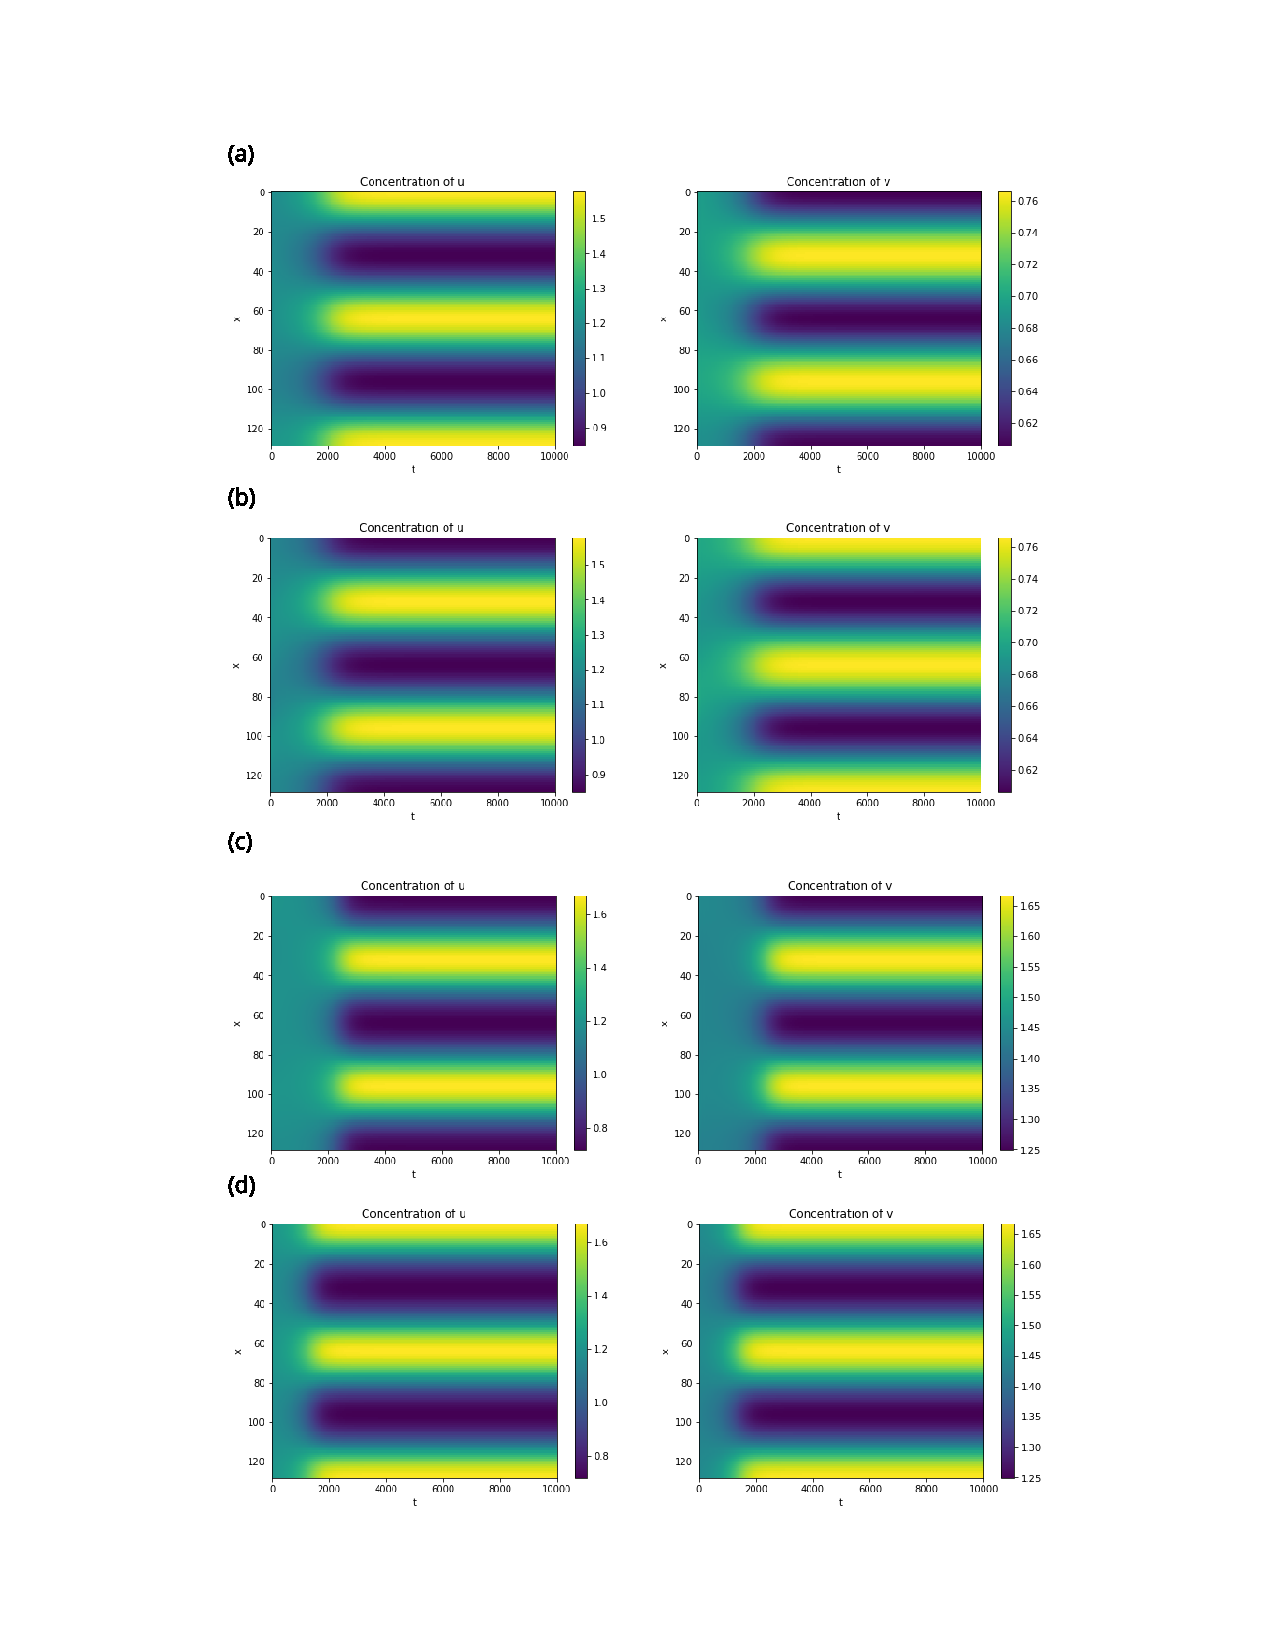
\includegraphics[scale = 0.6]{Fig_1.pdf}
  \caption{Modal configurations for Schnakenberg (a,b) and Gierer-Meindhart (c,d) systems. All simulations have $a = 0.2$, $b = 1$, $\gamma = 500$, $D_1 = 1$ and $D_2 = d_c + 2$. The selection of modal configuration in the system depends on the initial random perturbation. Patterns will persist in their chosen configuration for the duration of the simulation.}
\end{figure}
\end{center}
\section{Patterning in stochastic systems}

This section will investigate the key differences between pattern formation in stochastic and deterministic systems. To aid the analysis of such systems, two methods of quantifying pattern formation will be introduced in \textsection 6.1. Following this, the mathematics driving pattern formation in stochastic systems will be discussed in \textsection 6.2, looking in particular at the behaviour of the Turing bifurcation point. 

Sample simulations will be presented in \textsection 6.3, allowing us to see the behaviour of these systems near the bifurcation point. All simulations in this section were produced via the methods described in \textsection 4.

\subsection{Quantifying pattern formation}

The heat maps used in \textsection 5 are a useful tool for highlighting the pattern forming properties of deterministic systems. They are able to clearly show when a system is in pattern forming regime, and when transitions between regimes occur. However, when we introduce stochasticity to the systems it is not always clear when patterning is occurring. As we will see later in this chapter, stochastically driven reaction diffusion systems often display frequent jumping between strongly and weakly patterned states, as well as periods of relative spatial homogeneity, making heat maps more difficult to interpret. As such, it will be useful to consider a way of quantifying pattern forming behaviour. 

An approach used in \cite{Zheng-Ping} provides a useful method of quantifying the relative intensity of pattern formation. This dissertation employs a similar method, adapted to suit one-dimensional systems. The variable $\rho (t)$ acts as a measure of the overall spatial homogeneity of the system. It is calculated as the sum of the variance squared at each time step. Hence we have:

\begin{equation} \label{rho}
    \rho (t) = \sum_{j=1}^J \left(u_j - \frac{1}{J}\sum_{j=1}^J u_i\right)^2.
\end{equation}

Where $J$ is the number of spatial bins used in the simulation. The value of $\rho$ at a particular time will tell us whether the system is exhibiting pattern forming behaviour, as well as the relative amplitude of that pattern forming behaviour. By considering the way $\rho$ changes over the period of the simulation we can also gain some insight into the relative stability of patterns formed.

The stochasticisty present in the systems can lead $\rho$ to vary significantly between subsequent time steps. As such a moving average is used to aid the interpretation of results. This algorithm takes the average value of $\rho$ across the previous 100 steps and the proceeding 100 steps. At steps $n<100$ the average is only calculated from the proceeding 100 steps, and for $n>N-100$ the average is taken over only the preceding 100 steps. 

In addition to this measure of patterning intensity, it will also be useful to identify the modal frequency of the patterning. In the deterministic case this is as simple as counting how many peaks and troughs there are in the simulated results, however, this becomes more difficult when we factor in stochastic noise.

The mode counting algorithm used in this dissertation has two steps. First, the pattern is modified so that, at each time step, any value greater than the mean is assigned the value one, and any value lower than the mean is assigned the value zero. Letting $\bar{u}^n$ be the mean value of $u$ at time step $n$, and $\hat{u}_j^n$ be the modified $u$ at point $j$ and time $n$, we have the following:

\begin{equation}
 \hat{u}_j^n =  \left\{
\begin{array}{ll}
      0 & \text{for} \quad u_j^n<\bar{u}^n \\
      1 & \text{for} \quad u_j^n\geq\bar{u}^n. \\
\end{array} 
\right.
\end{equation}

This has the effect of 'sharpening' the output and gives well defined transitions between peaks and troughs. The next step is to count these transitions. This is achieved by subtracting the value of $\hat{u}_j^n$ from $\hat{u}_{j+1}^n$ and taking the absolute value of the result. Hence, if there is no transition present then the corresponding element has value zero, while at a transition it has value one. Each element of the resulting vector is then added up to give the total number of transitions. Hence, the number of modes at time $n$ is denoted $m_n$, where:
\begin{equation}\label{ModeAlg}
    m_n = \sum_{j=1}^{J-1} \left|\hat{u}_j^n - \hat{u}_{j+1}^n\right|.
\end{equation}

The output of this algorithm will be a vector of length equal to the number of time steps of the simulation. In stochastic systems we will see patterning of only one mode, however as the system falls into homogeneous periods there will be an increase in the number of transitions picked up by the algorithm. Plotting the number of modes as a histogram will result in a spike around the main mode of patterning, with any variance indicating that the simulation has spent time in more homogeneous periods. Hence, a taller, sharper histogram indicates more consistent patterning, while a shorter, wider histogram indicates less stable patterning. 
\subsection{Linear stability analysis in stochastic systems}
As with the deterministic case, the identification of a Turing bifurcation point in stochastic systems requires that the system is first linearised. The proceeding section will focus on pattern formation in systems of PDEs with a demographic white-noise term. For the reasons discussed in \textsection 3, that is the potential occurrence of non-positive values with additive noise, the simulations in this section will feature multiplicative noise terms. Hence, these equations will be of the form:

\begin{equation} \label{spde1}
d u(x,t) = [D_1\Delta u(x,t) + f(u,v)]d t + c_1\cdot u(x,t) 
d W(x,t),
\end{equation}
\begin{equation} \label{spde2}
d v(x,t) = [D_2\Delta v(x,t) + g(u,v)]d t+  c_2\cdot v(x,t) d W(x,t).
\end{equation}
The system is subject to Neumman boundary conditions, and the initial conditions are given by:

$$u(x,0) = u_0, \quad v(x,0) = v_0.$$
The deterministic non-linearities correspond to the Schnakenberg and Gierer-Meindhart systems described in (\ref{ScFunc}-\ref{AIFunc}). 

The pattern forming properties of this type of system are investigated in \cite{Zheng}. Zheng et al. consider the system with $\sigma_1 = c_1 \cdot( u - u_{\ast})$ and $\sigma_2 = c_2 \cdot(v - v_{\ast})$, where $f(u_{\ast}, v_{\ast}) = g(u_{\ast},v_{\ast}) = 0$, and $c_i$ are positive constants. These values were chosen to ensure that the amplitude of the stochastic noise goes to zero when the system is in a steady state. A benefit of treating $\sigma$ in this way is that it allows for the stochastic system to be easily linearised. By doing this, Zheng et al were able to show that the variance of the stochastic process provides a contribution to the linearisation matrix. 

The approach taken in \cite{Zheng} was to treat the demographic noise as a normally distributed random variable with mean zero and standard deviation $s$. By doing this they arrived at the following PDE describing the concentration of $u$:

\begin{equation} \label{spde1}
\frac{\partial u(x,t)}{\partial t} = D_1\Delta u(x,t) + f(u,v) + \frac{c_1\cdot(u - u_\ast)}{\sqrt{2\pi}s}\cdot\exp{-\frac{(u-u\ast)^2}{2s^2}} 
\end{equation}

Introducing a small perturbation from the steady state, $\tilde{u} = u - u_\ast$, and performing the usual Taylor expansion and linearisation leaves the following:
\begin{equation}
\frac{\partial \tilde{u}(x,t)}{\partial t} = D_1\Delta \tilde{u}(x,t) + \tilde{u}\cdot f_u + \tilde{v}\cdot f_v + \tilde{u}\cdot\frac{c_1}{\sqrt{2\pi}s}.
\end{equation}

The same techniques can then be applied to \eqref{spde2} to obtain a similar PDE describing the concentration of $v$. Following the usual techniques described in \cite{Murray, Turing, Britton}, Zheng et al. arrived at the following linearisation matrix:

\begin{equation}\label{Zhenglinsys}
    \frac{\partial}{\partial{t}} 
    \left(
    \begin{array}{c}
    u\\
    v\\
    \end{array}
    \right)
    = 
    \left[
    \begin{array}{cc}
      f_u - k^2D_1 + \frac{c_1}{\sqrt{2\pi}s}   & f_v \\
      g_u   &  g_v - k^2D_2 + \frac{c_2}{\sqrt{2\pi}s}
    \end{array}
    \right]
    \left(
    \begin{array}{c}
    u\\
    v\\
    \end{array}
    \right)
\end{equation}

However, it is not always appropriate to make the same choice for $\sigma$ as used in \cite{Zheng}. In many real life systems we see stochasticity destabilising a steady state (see e.g. \cite{Smolen}), and it is this type of system that we will be investigating in this dissertation, hence the choice of $\sigma_1 = c_1\cdot u(x,t)$ and $\sigma_2 = c_2\cdot v(x,t)$ in (\ref{spde1}-\ref{spde2}).

For the multiplicative noise investigated in this section, the linearisation of the stochastic PDE is not as neat as in \cite{Zheng}, however we may still assume that there will be some random variable related to the initial stochastic process present in the linearised matrix. Denoting this random variable $\xi_i$, our linearised matrix becomes:

\begin{equation}\label{stochlinsys}
    \frac{d}{dt} 
    \left(
    \begin{array}{c}
    u\\
    v\\
    \end{array}
    \right)
    = 
    \left[
    \begin{array}{cc}
      f_u - k^2D_1 + \xi_1   & f_v \\
      g_u   &  g_v - k^2D_2 + \xi_2
    \end{array}
    \right]
    \left(
    \begin{array}{c}
    u\\
    v\\
    \end{array}
    \right)
\end{equation}

The linearised matrix \eqref{linsys} is the foundation on which the Turing bifurcation analysis is built in the deterministic case. As such, it would be reasonable to assume that the random variables introduced in \eqref{stochlinsys} might have some influence on the capacity for the system to form patterns. In the next section we will see that this stochasticity has a variety of effects on the rate at which systems fall in to spatially patterned regimes, the stability and persistence of these regimes, and the influence of the critical diffusivity constant, $d_c$.

\subsection{Stochastic effects near the Turing bifurcation point}

In \textsection 5.2 we identified a critical diffusion constant for which patterning can occur in deterministic systems. This critical value was derived from the four diffusion driven instability conditions, which were in turn derived from the linearised system \eqref{linsys}. In the stochastic case, however, we have seen that this linearised system is quantitatively different.

The discrepancies between \eqref{linsys} and \eqref{stochlinsys} are reflected in the value of the critical diffusivity constant, $d_c$, for each system. In the stochastic case described by \eqref{stochlinsys} we now have:

\begin{equation}\label{stochdc}
 d_c = \frac{(f_vg_u - f_u^*g_v^*) \pm \sqrt{(f_vg_u-f_u^*g_v^*)^2 - (f_u^*g_v^*)^2 }}{f_u^*^2}.
\end{equation}
Where $f_u^* = f_u + \xi_2$ and $g_v^* = g_v + \xi_1$. Hence, we have that the stochastic process in (\ref{spde1} - \ref{spde2}) interferes in some way with the Turing bifurcation point. When the diffusivity constant is near the critical value, this interference presents itself in four ways:

\begin{enumerate}
    \item [(i)] patterning is possible in systems with sub-critical diffusivity constants,
    \item [(ii)] patterns produced with super-critical diffusivity constants can be of significantly higher intensity than in corresponding deterministic systems,
    \item [(iii)] the patterns formed lack stability, regularly falling into periods of relative homogeneity,
    \item[(iv)] partnering spontaneously switches between corresponding modal configurations. 
\end{enumerate}

Figure 2 shows the averaged outcomes of 20 simulations of the Schnakenberg stochastic reaction diffusion system for different values around the bifurcation point, with varying amplitudes of multiplicative noise. The distance from the deterministic critical diffusion constant is given by the parameter $\varepsilon$, i.e we have that $d_1 = 1$ and $d_2 = d_c + \varepsilon$. Hence, negative values of $\varepsilon$ correspond to a sub-critical diffusivity constant, and a larger magnitude of $\varepsilon$ corresponds to a value further from the bifurcation point.  

Accompanying each heat map is a chart showing the change in patterning intensity, $\rho$, through the course of the simulation, as calculated in \eqref{rho}, as well as a histogram of the modes present in the system, as calculated in \eqref{ModeAlg}. 

\begin{figure}
  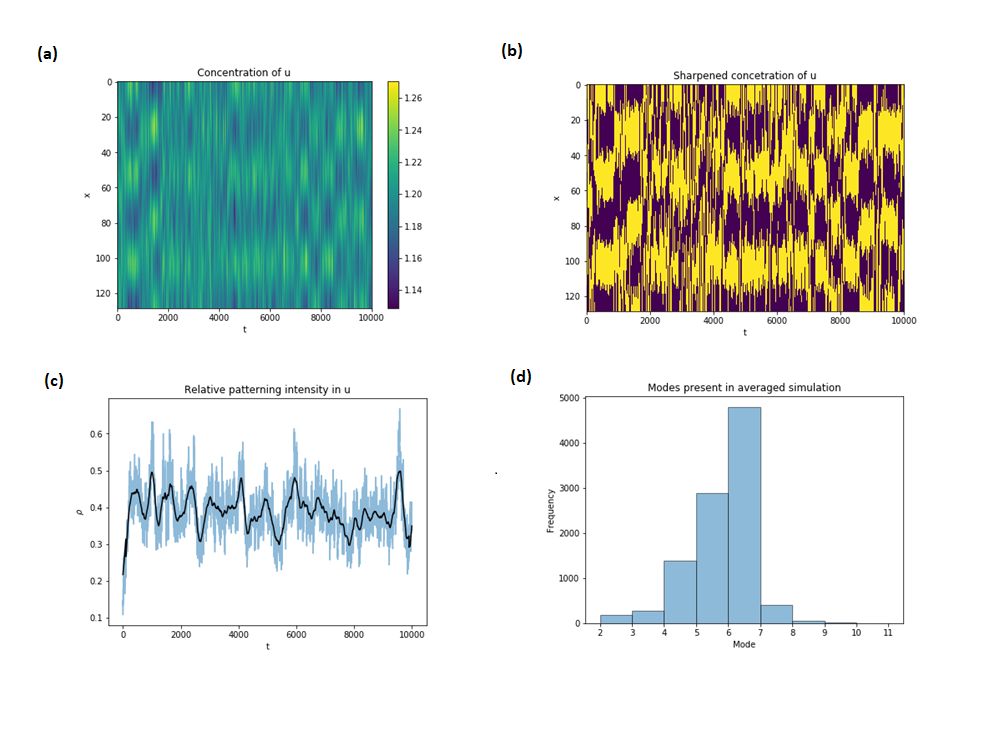
\includegraphics[scale = 0.65]{Fig_2.png}
  \caption{Averaged outputs for 20 simulations of the Schnakenberg system with multiplicative noise. All simulations have $a = 0.2$, $b = 1$, $\gamma = 800$, $\varepsilon = -0.1$, $c_1 = c_2 = 0.1$. The parameters for approximating the deterministic part of the system and for simulating sample paths of the stochastic process are as described in \textsection 4. (a) shows patterning present in the u equation, which is highlighted in the sharpened image (b) as described in \textsection 5.1. (c) shows the change in patterning intensity through the course of the simulation, displaying clear periods of relatively stable patterning, interspersed with frequent homogeneous periods. The central black line in this plot is a moving average calculate from the nearest $\pm 100$ time steps. (d) shows the modes present in the averaged result. We can see that the most common mode is 6, as is expected from the deterministic system. The presence of alternate modes indicate that the system is experiencing instability in the patterns formed.}
\end{figure}

The emergence of patterning in sub-critical systems is shown in figures 2(a-d). We can clearly see that, despite patterning being prohibited in the deterministic case, the system is still able to fall into a pattern forming regime, in agreement with a number of other papers (e.g. \cite{Zheng-Ping, Biancalani, Karig}). This phenomenon is due to small changes in the bifurcation point occurring as a result of the stochastic influence shown in \eqref{stochdc}. 

Figure 2(c,d) highlight the lack of stability present in the simulated patterns. The value of $\rho$ varies significantly through the course of the simulation, indicating frequent periods of weaker patterning. This is again highlighted in the histogram of modes present in the simulation. We can see that there are no major shifts in modal frequency of patterning, but we still see a wide number of modes present in the histogram. This indicates that the are frequent periods in which the noise in the system is dominating, leading to spells of relative homogeneity.

\begin{center}
\begin{figure}
  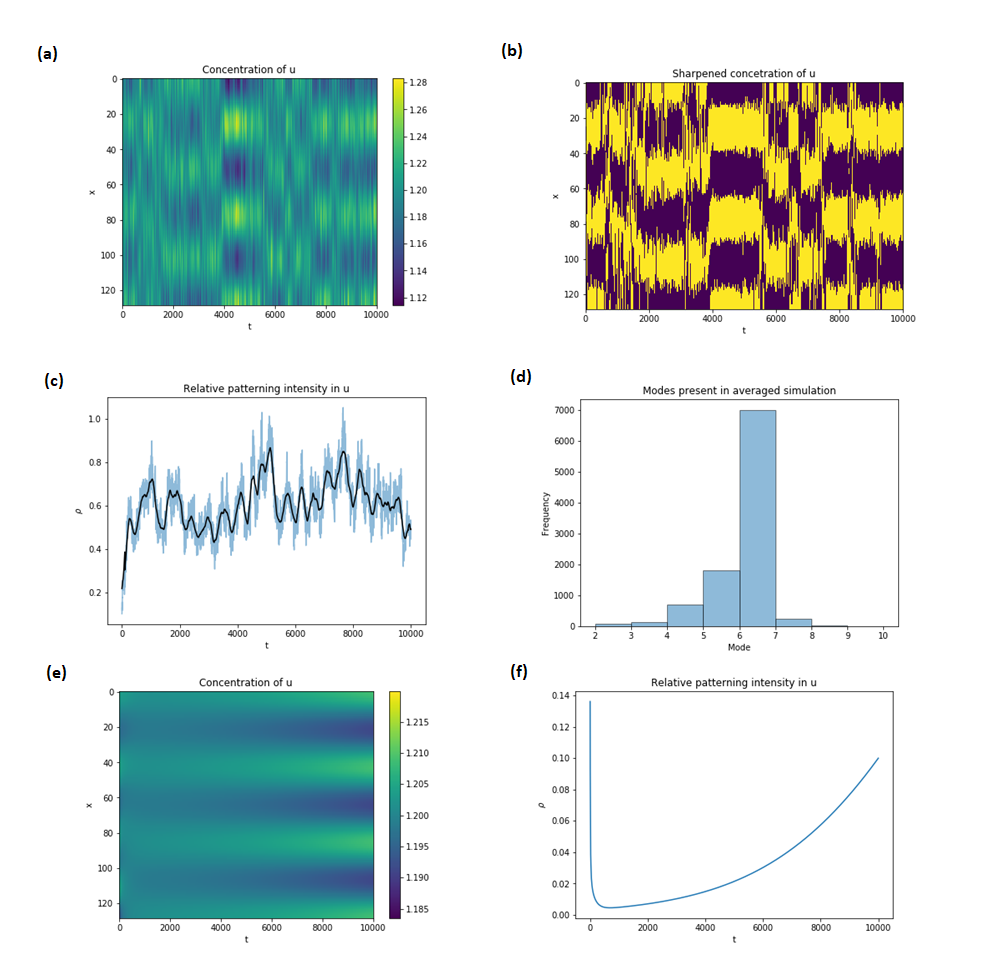
\includegraphics[scale = 0.65]{Fig_3.png}
  \caption{Averaged outputs for 20 simulations of the Schnakenberg system with multiplicative noise (a-e), and an equivalent deterministic system (e,f). All simulations have $a = 0.2$, $b = 1$, $\gamma = 800$, $\varepsilon = 0.1$. For (a-d) we have $c_1 = c_2= 0.1$, while (e,f) are deterministic systems. The parameters for approximating the deterministic part of the system and for simulating sample paths of the stochastic process are as described in \textsection 4. (a) shows patterning present in the $u$ equation, again this is highlighted in the sharpened image (b). This simulation displays similar characteristics to that of figure 2, although the patterns appear more stable. (c) The average patterning intensity is stronger than in the sub-critical case, and significantly stronger than in the deterministic case, shown here in (e,f). Note that the initial spike in $\rho$ in (f) is an artifact of the initial perturbation of the system. The distribution of modes shown in (d) indicates that switching to relatively homogeneous states is less common in super-critical systems as in the sub critical systems displayed in figure 2.}
\end{figure}
\end{center}
Figure 3(a-d) shows the pattern forming behaviour of the stochastic system just past the bifurcation point, while figure 3(e,f) represents a simulation of the corresponding deterministic system.  This highlights several interesting features of stochastic pattern formation. 

When the system is in a patterned state the value of $\rho$ is consistently significantly higher in the stochastic system than in the deterministic system. This indicates that much more intense patterning is possible for stochastic systems near the bifurcation point. This is likely the result of Fourier modes in the demographic white noise which promote the growth of patterned frequencies. Similar results can be seen in \cite{Zheng-Ping}.

This process also causes notable behaviour at the onset of patterning. In deterministic systems we see a period of homogeneity before settling into a stable patterned regime, as shown in figure 1 and figure 3(e), while it is clear from these simulations that in stochastic systems we see a much more abrupt transition, and much less stability in the patterns formed. 

In both cases, the loss of patterning stability is again driven by small changes in the bifurcation point of the system. Comparing figure 2(d) and 3(d) we can see that the super-critical simulation spends more time in the 6-mode patterning regime, indicating more stable patterning. This is because the super-critical simulation is further into the 'safe-zone' for patterning, so stochastic perturbations are less likely to cause a loss of stability. 

Spontaneous switching between modal configurations occurs in both figures 2 and 3. It is important to note that the mode of the patterning does not change, just the location of the peaks and troughs. This phase shifting occurs after loss of patterning stability, causing the system to return to a homogeneous state. Resetting the system in this way means that either modal configuration is once again possible, so phase shifts can occur. This is again evident when we consider that phase-shifts become significantly less frequent as we progress further into the deterministically permitted patterning parameters. This process has also been demonstrated in \cite{Maini}. 

The simulations investigated in this section have highlighted the significance of stochastic noise on systems which are near the Turing bifurcation point. As we move further away from this point the observed effects are reduced and we see the return of much more stable patterned regimes. Intuitively, this is because the influence of $\xi$ in the linearised system becomes relatively small and can not significantly influence the location of the bifurcation point.

In \textsection 7 we will see that stochastic forcing of model parameters, through what are known as \textit{random partial differential equations}, can result in changes in modal frequency of patterning. This result was not possible with the white-noise driven stochastic PDEs investigated in this section, and could help to explain some of the regime shift we observe in patterned systems in biology.

\section{Random partial differential equations}
In previous sections we have dealt with systems of stochastic partial differential equations which are typified by the inclusion of a demographic white-noise term. We have seen the role this stochasticity plays in modulating the Turing bifurcation points of such systems, and the effects of this modulation on a system's pattern forming characteristics. However, stochastic differential equations of the form (\ref{spde1}-\ref{spde2}) were unable to capture the mode changing behaviour often seen in biological systems. 

To investigate this process further we must return to the scaling parameter $\gamma$ introduced in \textsection 2. We will begin by exploring the role $\gamma$ plays in pattern formation, in particular in the determination of the modal frequency of patterning. In \textsection 7.2 we will introduce a family of stochastic systems, known as \textit{random partial differential equations}, in which a given parameter undergoes stochastic forcing. Finally, in \textsection 7.3 we will show that simulations of these systems display spontaneous shifting into patterns of alternate modal regimes.


\subsection{The role of $\gamma$ in mode selection}
We have seen that for deterministic systems, patterns will form with wavenumbers which (a) are permitted by the domain, and (b) correspond to the most unstable eigenvalue in the dispersion relation. The patterns which are permitted are decided by both the size of the domain and the values of model parameters. 

The parameter $\gamma$ plays an important role in mode selection by scaling the non-linearites relative to the diffusion rate. Figure 4g shows the effect of gradually increasing $\gamma$ in the schnakenberg model. Here, we can see that regime shifts into different modal frequencies occur at very specific $\gamma$ values. We will later see that near these values, any stochasticity in $\gamma$ can result in spontaneous regime shifts in the system.

\begin{figure}
\begin{center}
  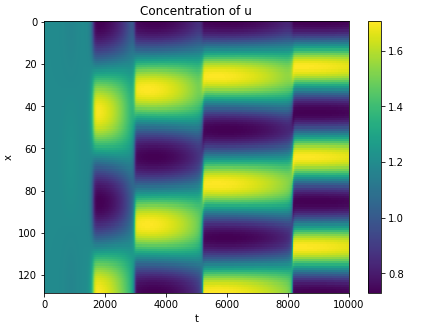
\includegraphics[scale = 0.65]{Fig_4.png}
  \caption{Patterneing produced in a deterministic Schnakenberg system with $\gamma$ gradually increased at a rate $\gamma(t) = (N/1500)t + \gamma(0)$, with initial value $\gamma(0) = 100$. The parameterisations were $a=0.2$, $b=1$, $\varepsilon = 3$. The simulation was performed using the discretisations described in \textsection 4. }
  \end{center}
\end{figure}
\subsection{Accounting for randomness in $\gamma$}
Random reaction diffusion equations attempt to model uncertainty in the parameter values of their deterministic counterparts. To achieve  this we employ a method demonstrated in \cite{Zhonghuai}. The random variable $\xi \sim \mathcal{N}(0,1)$ is introduced, and is permitted to modulate the target parameter. In the case that we are modulating the parameter $\gamma$ in the system (\ref{dpde1}-\ref{dpde2}), we have: 

\begin{equation} \label{StochGamma1}
\frac{\partial u(x,t)}{\partial t} = D_1\Delta u(x,t) + (\gamma + \sigma_s\xi(x,t)) \cdot f(u,v),
\end{equation}
\begin{equation} \label{StochGamma2}
\frac{\partial v(x,t)}{\partial t} = D_2\Delta v(x,t) + (\gamma + \sigma_s \xi(x,t)) \cdot g(u,v).
\end{equation}

where $\sigma_s$ modulates the variance of the random variable $\xi$. The Neumann boundary conditions and initial conditions remain unchanged. In the interest of brevity, the notation $r=\gamma +\sigma_s\xi$ will be used for the remainder of this dissertation. 

This new stochastic parameter, $r$, still has the effect of scaling the model parameters, and as such the uniqueness and existence results from \textsection 2.3 still apply. Rigorous mathematical analysis of this type of equation is outside the scope of this paper, however the reader is referred to \cite{Lu} for an investigation into the controlability of such systems, and \cite{Gittelson} for a demonstration of the well-posedness of weak-formulations of the problem, and a suggested Galerkin discretisation approach.

Care must be taken to ensure that $r$ remains positive throughout the duration of the simulation. If the quantity becomes negative then the nature of the non-linear function changes, altering the stability properties of the system and potentially disrupting the boundedness of the problem. It is tempting to avoid this problem by introducing a multiplicative element to the parameter $\sigma_s$, however this also affects the nature of the non-linearity and can lead to similar problems. In practice, the best course of action is to limit the variance of the stochastic process. 

Since $\xi$ is a normally distributed random variable, we can assume that over the course of $N=10,000$ time steps, the value of $r$ will be unlikely to vary by more than $\sqrt{\Delta t}\cdot N$. Hence, we can expect $r$ to remain roughly within $r \approx \gamma \pm \sigma_s \cdot 100$. Clearly, the acceptable size of $\sigma_s$ will depend on the number of time steps in the simulation and the initial value of $\gamma$. For a simulation of 10,000 steps, with $\gamma = 1200$, then $0 \leq \sigma_s \leq 5$ should be sufficient to avoid negative values.

\subsection{Pattern formation in random partial differential equations}

The simulations performed in this section are calculated using the implicit finite difference method described in $\textsection 4.2$ and A1. The random variable $\xi \sim \mathcal{N}(0,1)$ is simulated via the introduction of a normally distributed random variable. At each time step, the stochastic process is approximated by averaging over 10 realisations of $\xi$, as was the case for the simulation of stochastic partial differential equations. 

The time and space discretisation in each simulation are $\Delta t = 10^{-4}$ and $\Delta x = 1/128$, with $t \in [0,1]$ and $x \in [0,1]$, unless otherwise stated. The parameters are set at $a = 0.2$, $b = 1$ and $\gamma = 1200$. To avoid any influence from simulating near the Turing bifurcation point, all simulations have $\varepsilon = 1$. 

In order to investigate the time and space dependence of $\xi$, two cases are considered: 
\begin{enumerate}

    \item [(i)] $\xi(t)$ varies across the time period, but is independent of location. This corresponds to a global change in the amplitude of $\gamma$, modelling the effect of, for example, climate, temperature or pH. 
    \item[(ii)] $\xi(x,t)$ is dependant on both time and location. This could correspond to genetic variations in an ecological system, or extraneous chemical reactions in a biochemical system.  
\end{enumerate}

\subsubsection{Patterning when $\xi(t)$ varies with time only}
Allowing $\xi$ to vary with time results in a system that spontaneously shifts into alternate modes through the course of a simulation. Figure 5(a) shows the output of a single simulation with a time dependent $\xi(t)$, with 5(b) showing the corresponding $\rho$ as discussed in the previous section. Figure 5(c) shows the value of $r$ at each time step. Several interesting effects can be seen in this simulaiton. 

Firstly, it is clear that by allowing $r$ to vary over time we are able to produce spontaneous shifts in the modal frequency of patterning. These shifts occur when $r$ crosses a certain threshold value, as was the case in the deterministic simulaiton shown in figure 4.   

It is notable that the value of $r$ required for a shift down in modal frequency is not necessarily the same value required for a return to the previous regime. At around $t \approx 3500 \Delta t$ we see a transition from mode 7 to mode 6 patterning, corresponding to $r$ passing through $r \approx 900$. However, when $r$ passes the same value in the other direction we do not observe a shift back to mode 7 patterning, with this shift only occurring when $r \approx 1200$. This indicates that when the system enters a new patterning regime, a change back to the original parameters does not necessarily correspond to a return to the original regime, hence the system is displaying hysteresis during regime shifts.  
\begin{figure}
\begin{center}
  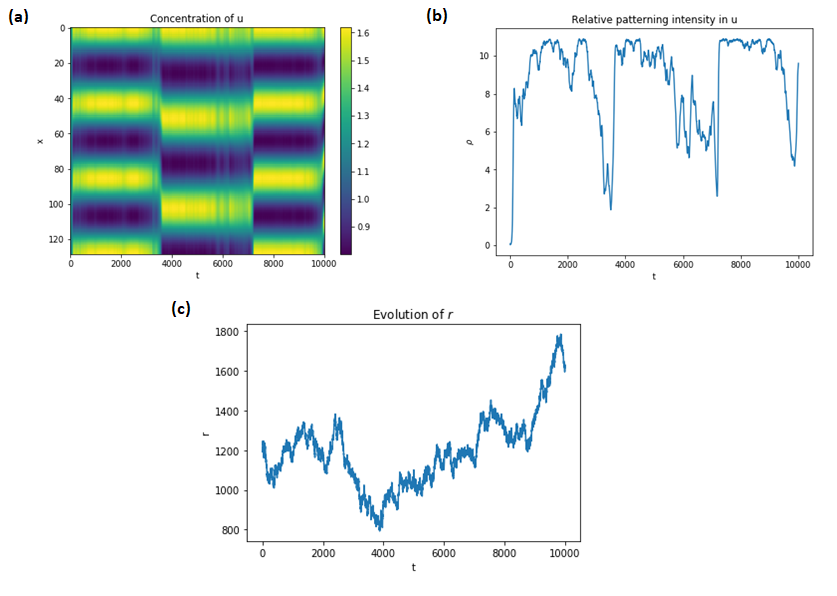
\includegraphics[scale = 0.75]{Fig_5.png}
  \caption{Patterneing produced in a random Schnakenberg system with $\xi(t)$ permitted to vary in time only, with $\sigma_s = 2$. (a) Shows the development of the pattern through the simulation, we can clearly see mode changes at $t \approx 3500\Delta t$ and $t \approx 7000\Delta t$. (b) shows the evolution of $\rho$ through this process, demonstrating a gradual loss of patterning intensity prior to a mode change. In (c) we see that mode changes appear to occur when $r$ passes through certain thresholds, and that this process has hysteric properties.}
  \end{center}
\end{figure}

Figure 5(b) demonstrates a potential early warning sign for these regime shifts. In the moments leading up to a shift of mode the patterning intensity gradually drops, before qucikly returning to its original levels after the transition occurs. In systems in which the value of $r$ is difficult to measure, this loss of patterning intensity could act as a tool for predicting regime shifts. A similar increase in noise before regime shifts in stochastic partial differential equations is highlighted in \cite{Gowda}. 

\begin{figure}
\begin{center}
  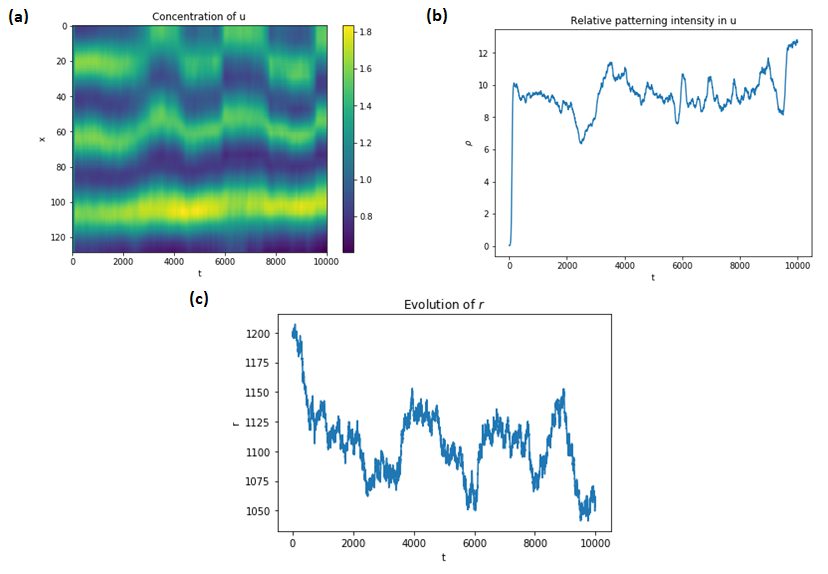
\includegraphics[scale = 0.75]{Fig_6.png}
  \caption{Patterning produced in a random Schnakenberg system with $\xi(x,t)$ permitted to vary in time and space, with $\sigma_s = 5$. (a) Shows the development of the pattern through the simulation. We can see that the positioning of the patterns gradually shifts over time, and mode shifts are much less abrupt than in figure 5(a). The evolution of $\rho$ during the simulation, shown in (b), is far less varied than in the non-spatially dependant case. In (c) we see that the variation in $r$ is considerably smaller than in figure 5(c).}
  \end{center}
\end{figure}

\subsubsection{Patterning when $\xi(x,t)$ varies with position and time}
Figure 6 shows a typical simulation in which $\xi$ is permitted to vary with both time and space. Three key results can be inferred from this simulation:
\begin{enumerate}
\item[(i)] The spatial distribution of peaks and troughs in the patterning is less well defined, as shown in 6(a). This results in patterns with less symmetry than was the case with demographic white noise.  
\item[(ii)] Transitions between modal regimes are more fluid than in the spatially independent case. Figure 6(b) indicates that patterning intensity remains relatively consistent through transitions, without the dramatic loss of patterning seen in Figure 5. These modal shifts also appear to be localised. Note that the mode shift at $t\approx3000\Delta t$ has a significantly larger contribution from the upper stripe than from the lower stripe. 
\item[(iii)] With $r$ now distributed across 128 spatial points, the average value of $r$ during the simulation varies significantly less than in the spatially independent case, as highlighted in 6(c). This results in less frequent mode changes since it is the average value of $r$ which drives modal regime shifts. 
\end{enumerate}

The patterns formed from simulating reaction diffusion systems in which the model parameter $\gamma$ is permitted a degree of stochasticity in both position and time are qualitatively similar to the patterns observed in nature. They reflect the slight asymmetries seen in coat markings, as well as the gradual spatial drift of animal territories, or small irregularities in gene expression. As such, this method is a useful tool for gaining a deeper insight into the pattern forming properties of reaction diffusion systems.

\section{Discussion}
The aim of this dissertation was to demonstrate the effects of stochastic noise on the pattern forming properties of reaction-diffusion systems. To achieve this we have demonstrated the well-posedness of systems with demographic white noise, developed a method for simulating such systems, and uncovered some of the important properties of noisy pattern formation. In doing this, we have tied together two key areas of current research in the mathematics community, that of pattern formation and of stochastic simulation. As such, there are a wealth of possible routes for further investigation.  

The development of quasipatterns is a result which is particularly significant, as it broadens the scope of possible applications of the theory, as highlight by a number of papers (e.g \cite{Karig, Biancalani, Butler}). This dissertation has focused solely on the bifurcation point through the diffusivity constant, however it could be fruitful to see to what extent the effect occurs throughout the parameter space.   

In \textsection 5 we saw that patterned systems with demographic noise frequently fall back into a homogeneous state. This can pose a problem in biological systems, where the robustness of pattern formation is paramount. An investigation into the robustness problem can be found in \cite{Maini}, in which the effects of stochastic noise, boundary conditions and domain size are thoroughly investigated. An extension of this dissertation could look into the robustness problem, in particular looking at how far the system needs to be from a bifurcation point for robust patterns to occur.     

The occurrence of modal shifts in random partial differential equations is a very interesting result, and one which could certainly be investigated in further research. Recent research into the pattern forming properties of systems with stochastic parameters have accounted for rearrangement of vegetation in semi-arid ecosystems \cite{Siteur, chen}, with the random nature of parameters such as rainfall making good candidates for random perturbation. Any further investigation into this type of problem would benefit from more rigorous mathematical analysis, such as that found in \cite{Lu}, and a deeper consideration of the simulation methods employed, as shown in \cite{Gittelson}.     

From the perspective of stochastic simulation, it could be fruitful to investigate the effect the $Q$-Wiener process parameters have on pattern formation. This dissertation has focused on a specific value for the regularity, $r$, of the stochastic process. Investigating the pattern forming characteristics for different values of $0<r\leq 2$ could provide interesting results.

%Stochastic noise is often seen as an unattractive quality in a system. Its inherently disruptive nature is often the bane of scientists and engineers, who strive for clean signals and predictable outcomes. The results presented in this dissertation, however, have demonstrated another side to white-noise. We have seen that, under the right conditions, noise can be as much a creative force as a destructive one. It can explain why Turing-like patterns occur in otherwise prohibitive systems, why patterning onset can frequently be quicker than expected, and why spontaneous shifts in patterning symmetry occur. 

When Turing first publish his 1952 paper on pattern formation it was met with a degree of skepticism from the scientific community. Initial reservations highlighted the absurdity that the usually dissipative force of diffusion could be the foundation from which structure is born. It is fitting, then, that the paradox of order from chaos appears to once again be central in our modern mathematical analysis of the pattern forming problem. 
 
\printbibliography

\newpage
\appendix
\section{Appendix}
\subsection{Implicit finite difference method}
The numerical method described in \textsection 4.1 employs the following approximations of first order time and second order space derivatives:

\begin{equation*}
    \frac{du}{dt} \approx \frac{\delta_t u_j^n}{\Delta t} = \frac{u_j^{n} - u_j^{n-1}}{\Delta t},
\end{equation*}

\begin{equation*}
    \frac{d^2u}{dx^2} \approx \frac{\delta_x^2 u_j^n}{\Delta x^2} = \frac{u_{j+1}^n - 2u_j^n + u_{j-1}^n}{\Delta x^2}.
\end{equation*}
Hence, by letting $r_1 = D_1\Delta t / \Delta x^2$, the deterministic PDE \eqref{dpde1} is approximated by:

\begin{equation}\label{apend dpde appx}
    \left[2r_1 + 1\right]u_j^{n+1} - r_1\left[u_{j+1}^{n+1} + u_{j-1}^{n+1} \right]  = u_j^n + \Delta t \cdot f(u_j^n, v_j^n).
\end{equation}
This can be written as:

\begin{equation*}
    B_1\cdot u^{n+1} = u^n + \Delta t \cdot f(u^n),
\end{equation*}
where $B_1$ is as described in \textsection 4.1. The equation for $v$ is arrived at in a similar way.

Neumann boundary conditions are dealt with by employing a fictitious point method. The first order spatial derivative of $u$  is approximated by a central difference operator, such that:
\begin{equation} \label{apend fp method}
    \frac{du}{dx} \approx \frac{u_{j+1}^n - u_{j-1}^n}{\Delta x} = 0.
\end{equation}

By considering the boundary points $j = 0$ and $j = J$, and substituting \eqref{apend fp method} into \eqref{apend dpde appx}, we arrive at the following approximation at the boundaries:

\begin{equation}
    \left[2r_1 + 1\right]u_0^{n+1} - 2r_1\cdot u_1^{n+1}  = u_0^n + \Delta t \cdot f(u_0^n, v_0^n),
\end{equation}
\begin{equation}
        \left[2r_1 + 1\right]u_J^{n+1} - 2r_1\cdot u_{J-1}^{n+1}  = u_J^n + \Delta t \cdot f(u_J^n, v_J^n).
\end{equation}

These can then be incorporated into the matrix $B_1$ by setting $B_1(1,2) = B_1(J, J-1) = -2r_1$. The order of accuracy of this scheme can be calculated via Taylor expansions, as shown in \cite{Iserles}, along with a demonstration of the stability of the scheme. 
\subsection{Python script for approximating SPDEs}
The following code was written in Python 3.0. It has been adapted from an original MatLab code provided by Mariya Ptashnyk, and includes functions made available by Tony Shardlow \cite{Shardlow}, based on MatLab code provided in \cite{Lord}, namely the functions \texttt{icspde\_dst1}, \texttt{get\_onedD\_bj} and \texttt{get\_onedD\_dW}.

\lstinputlisting[language=Octave, 
caption=Octave sample code
]{SPDE_Solve.py}

\clearpage
\end{document}